%% ---------------------------------------------------------------------------
%% Agent-based Transport Demand Modelling for Calvados
%%
%% Build (see report/README.md):
%%   .\build.ps1        (Windows, uses local LaTeX or Docker)
%%   ./build.sh         (Linux / macOS / Git Bash)
%% Output: build/main.pdf
%% ---------------------------------------------------------------------------

\documentclass[a4paper, 11pt]{article}

%% ---------------------------------------------------------------------------
%% Packages, layout and macros. Content lives in chapters/, metadata in main.tex.
%% ---------------------------------------------------------------------------

%% Fonts and language
\usepackage[T1]{fontenc}
\usepackage{lmodern}
\usepackage[english]{babel}
\usepackage{microtype}

%% Layout
\usepackage[margin=2.5cm]{geometry}
\usepackage{indentfirst}
\usepackage{setspace}
\onehalfspacing
\emergencystretch=2em % avoid overfull lines with long names in monospace

%% Math
\usepackage{amsmath, amssymb, mathtools}

%% Figures and tables
\usepackage{graphicx}
\graphicspath{{figures/}} % 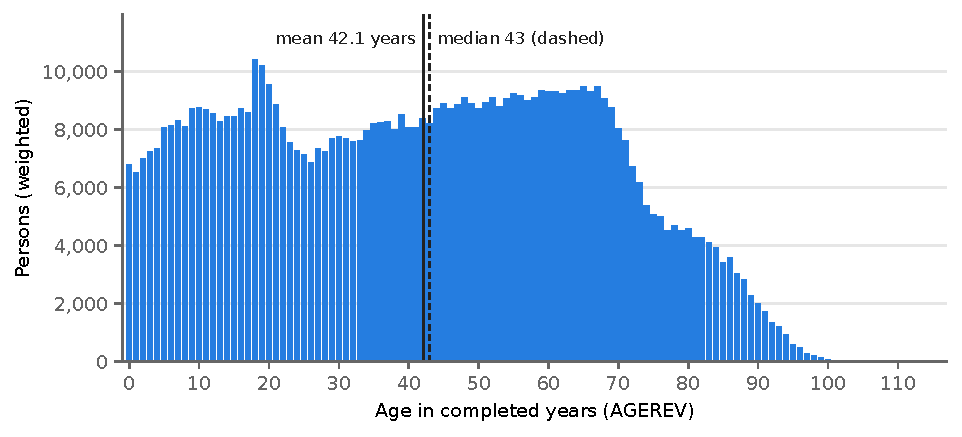
\includegraphics{age_distribution} -> figures/age_distribution.(pdf|png)
\usepackage{float}        % [H] placement
\usepackage{booktabs}
\usepackage{tabularx}
\usepackage{caption}
\usepackage{subcaption}
\usepackage{xcolor}

%% Algorithms and code listings
\usepackage{algorithm}
\usepackage{algpseudocode}
\usepackage{listings}
\lstset{
  basicstyle=\ttfamily\small,
  breaklines=true,
  frame=single,
  columns=fullflexible,
  keywordstyle=\color{blue!60!black},
  commentstyle=\color{gray},
  % listings is not UTF-8 aware: map the accented letters used in column names
  literate={é}{{\'e}}1 {è}{{\`e}}1 {à}{{\`a}}1 {ç}{{\c{c}}}1 {ô}{{\^o}}1 {É}{{\'E}}1,
}
% Python excerpts of the analysis: \begin{lstlisting}[style=py] ... \end{lstlisting}
\lstdefinestyle{py}{
  language=Python,
  basicstyle=\ttfamily\footnotesize,
  columns=fixed, basewidth=0.5em, keepspaces=true,
  stringstyle=\color{green!40!black},
  showstringspaces=false,
  aboveskip=0.6\baselineskip,
  belowskip=0.6\baselineskip,
}

%% Question / answer boxes: one per question of the assignment
\usepackage[most]{tcolorbox}
% \begin{qa}{<question as asked in the assignment>} <answer> \end{qa}
\newtcolorbox{qa}[1]{
  enhanced, breakable,
  colback=blue!3, colframe=blue!45!black, boxrule=0.6pt, arc=1mm,
  left=2mm, right=2mm, top=1mm, bottom=1mm,
  before upper={\textbf{Question.} \emph{#1}\par\smallskip\textbf{Answer.}\ },
}

%% Links -- hyperref must be loaded late, cleveref after it
\usepackage[hyphens]{url}
\Urlmuskip=0mu plus 1mu % let long data URLs stretch instead of running into the margin
\usepackage[hidelinks]{hyperref}
\usepackage[capitalise, noabbrev]{cleveref} % \cref{fig:x} -> "Figure 1"

%% ---------------------------------------------------------------------------
%% Macros
%% ---------------------------------------------------------------------------
\newcommand{\todo}[1]{\textcolor{red}{\textbf{[TODO: #1]}}} % visible placeholder
\newcommand{\code}[1]{\texttt{#1}}                          % file / identifier names

% Placeholder for a figure that a notebook will write to figures/<name>.pdf.
% Replace the call by \includegraphics[width=\textwidth]{<name>} once the file exists.
\newcommand{\figplaceholder}[2][0.9\textwidth]{%
  \fbox{\parbox[c][5cm][c]{#1}{\centering
    \todo{figure \texttt{\detokenize{#2}.pdf} not generated yet}}}}

%% Transport-demand notation (all usable in text mode as well)
\newcommand{\Oi}{\ensuremath{O_i}}                 % trips originating in zone i
\newcommand{\Dj}{\ensuremath{D_j}}                 % trips arriving in zone j
\newcommand{\Fij}{\ensuremath{F_{ij}}}             % flow from zone i to zone j
\newcommand{\dij}{\ensuremath{d_{ij}}}             % centroid distance i -> j [m]
\newcommand{\rhoij}{\ensuremath{\rho_{ij}}}        % friction term
\newcommand{\Oprime}{\ensuremath{O'_i}}            % scaled origins (Exercise 2.2)
\newcommand{\pii}{\ensuremath{p_i}}                % production weighting factor
\newcommand{\aj}{\ensuremath{a_j}}                 % attraction weighting factor


%% ---------------------------------------------------------------------------
%% METADATA -- edit here
%% ---------------------------------------------------------------------------
\newcommand{\reporttitle}{Agent-based Transport\\Demand Modelling for\\Calvados}
\newcommand{\reportsubtitle}{From territorial analysis to routing on OpenStreetMap}
\newcommand{\coursename}{Large-scale models and simulation methods}
\newcommand{\institution}{Universit\'e Gustave Eiffel}
\newcommand{\academicyear}{2026/2027}
\newcommand{\repourl}{} % TODO: repository URL, leave empty to hide

\title{\reporttitle}
% The assignment requires ALL names and e-mail addresses on the report.
\author{%
  Ekaterina POPKOVA (\texttt{ekaterina.popkova@edu.univ-eiffel.fr}) \and
  Elham YAVUZ (\texttt{elham.yavuz@edu.univ-eiffel.fr})%
}
\date{\today}

\hypersetup{pdftitle={Agent-based Transport Demand Modelling}}

\begin{document}

\pagenumbering{roman} % front matter: i, ii, ...
%% Native title page (no precompiled cover PDF to keep in sync).
\makeatletter
\begin{titlepage}
  \centering
  \vspace*{2cm}
  {\large \institution\par}
  {\large \coursename\par}
  \vspace{3cm}
  {\Huge\bfseries \reporttitle\par}
  \vspace{0.8cm}
  {\Large \reportsubtitle\par}
  \vspace{2.5cm}
  % Outside \maketitle, \and is not usable as is: set the authors one per line ourselves.
  {\large \begin{tabular}[t]{c}\renewcommand{\and}{\\}\@author\end{tabular}}\par
  \vfill
  {\large \academicyear\par}
  \vspace{0.3cm}
  {\normalsize \@date\par}
  \ifx\repourl\empty\else
    \vspace{0.5cm}
    {\small \url{\repourl}\par}
  \fi
\end{titlepage}
\makeatother

\setcounter{page}{2} % titlepage environment resets the counter to 1; keep page labels unique

\tableofcontents
\clearpage
\pagenumbering{arabic} % body starts at 1

%% ---------------------------------------------------------------------------
%% CHAPTERS -- one file per section, in order
%% (comment a line out to exclude a chapter from the build)
%% ---------------------------------------------------------------------------
\section{Introduction}\label{sec:introduction}

\subsection{Goal of the project}
The goal of this project is to set up an agent-based transport demand pipeline for one French department outside
the \^Ile-de-France region. The pipeline starts with a territorial analysis of the study area, generates and attracts
trips per zone, distributes them with a double-constrained gravity model, disaggregates the resulting flows into
individual trips with coordinates and departure times, and finally routes these trips on a road network extracted from
OpenStreetMap. The simulation does not aim to be correct; it shows that the tools can be chained and that analyses can
be performed on their outputs.
\todo{Rewrite the goal in the authors' own words, 4--6 sentences, and add a short overview figure of the pipeline if useful.}

\subsection{Study area}
\todo{Name the chosen department (code and name), its location, its main urban centres and the reasons for the choice
(size, availability of data, a mix of urban and rural municipalities, \dots). The detailed census figures belong to
\cref{sec:study-area}.}

\subsection{Data sources}\label{sec:data-sources}
The following data sets are used (links, file names and known pitfalls are listed in \code{data/DATA\_SOURCES.md} of the
repository):
\begin{itemize}
  \item the INSEE detailed census, ``Individus localis\'es au canton-ou-ville'' \cite{insee-census-detailed};
  \item the INSEE aggregated census, ``Population en 2019 -- IRIS'' \cite{insee-census-aggregated};
  \item the IGN CONTOURS-IRIS boundaries, 2021 edition \cite{ign-contours-iris};
  \item the URSSAF number of employees per municipality and economic activity (APE) \cite{urssaf-employment};
  \item the OpenStreetMap extract of the region from Geofabrik \cite{geofabrik-osm}.
\end{itemize}
\todo{Add vintages, access dates and the exact files used. Mention that the detailed census is localised at the level of
``canton-ou-ville'' and not at municipality level (see \cref{sec:study-area}).}

\subsection{Tools}
The analysis is written in Python (geopandas \cite{geopandas}, OSMnx \cite{osmnx}, pyrosm \cite{pyrosm}) in Jupyter
notebooks, supported by a small shared package \code{lsm} in \code{src/}. The report is written in \LaTeX{}.
\todo{State the exact versions (taken from \code{environment.yml}) and refer to \cref{sec:appendix-reproducibility}.}

\subsection{Team split}
\Cref{tab:team-split} summarises who is responsible for which exercise. The only interface between the two parts is the
file \code{data/processed/zones.parquet} (zone identifier, name, geometry, \Oprime{}, \Dj{}), described in
\cref{sec:appendix-reproducibility}.

\begin{table}[H]
  \centering
  \caption{Team split. Points are those given in the assignment.}
  \label{tab:team-split}
  \begin{tabularx}{\textwidth}{@{}llXr@{}}
    \toprule
    Person & Name & Exercises & Points \\
    \midrule
    A & \todo{Name One} & 1.1 Study area, 1.2 and 1.3 Territorial analysis, 2.1 Trip production, 2.2 Trip attraction & 12 \\
    B & \todo{Name Two} & 2.3 Trip distribution, 3.1 Disaggregation, 3.2 Routing & 10 \\
    \bottomrule
  \end{tabularx}
\end{table}

\subsection{Structure of this report}
Each of \crefrange{sec:study-area}{sec:routing} answers one exercise of the assignment, one subsection per question, and
ends with the problems that were encountered. \Cref{sec:discussion} discusses limitations and consistency checks across
the pipeline.

\clearpage % the exercises start on a new page
\section{Study area (Exercise 1.1)}\label{sec:study-area}
\noindent Responsible: Person A. Notebook: \code{notebooks/A1\_study\_area.ipynb}.

\subsection{Number of observations, persons and municipalities (1 point)}

\paragraph{Method.}
\todo{Name the chosen department and justify the choice. Describe how the detailed census was filtered to the department
(zone file, department code, \code{IRIS} / \code{CANTVILLE} columns). Explain the three counts: (1) observations are rows
of the filtered file, (2) persons are the \emph{sum of the weights} \code{IPONDI}, not the number of rows, (3) municipalities
are counted from a source that identifies all of them. State how the municipalities without IRIS code in the detailed census
(small municipalities, localised only at ``canton-ou-ville'' level) are handled.}

\paragraph{Result.}
\todo{Report the three numbers, ideally in \cref{tab:study-area-counts}, and comment on the difference between observations
and weighted persons.}

\begin{table}[H]
  \centering
  \caption{\todo{Caption: census counts for the study area.}}
  \label{tab:study-area-counts}
  \begin{tabular}{@{}lr@{}}
    \toprule
    Quantity & Value \\
    \midrule
    Person observations (rows, unweighted) & \todo{value} \\
    Persons (sum of weights \code{IPONDI}) & \todo{value} \\
    Municipalities & \todo{value} \\
    \bottomrule
  \end{tabular}
\end{table}

\subsection{Map of the department inside of France (1 point)}

\paragraph{Method.}
\todo{Describe how the map is built from the IGN CONTOURS-IRIS 2021 data (dissolve to departments, highlight the study area,
projection EPSG:2154).}

\begin{figure}[H]
  \centering
  \figplaceholder{study_area_location}
  \caption{\todo{Caption: location of the study area inside of France.}}
  \label{fig:study-area-location}
\end{figure}

\paragraph{Result.}
\todo{Describe what \cref{fig:study-area-location} shows (neighbouring departments, main cities).}

\paragraph{Problems encountered.}
\todo{Document every problem for partial points: e.g.\ census files per zone, missing IRIS codes, municipality codes that
differ between sources, how they were resolved.}

\section{Territorial analysis I (Exercise 1.2)}\label{sec:territorial-I}
\noindent Responsible: Person A. Notebook: \code{notebooks/ex12\_territorial\_analysis\_I.ipynb}.

\paragraph{Data sources.}
Two census products are combined, and every number below states which one it comes from.
\begin{itemize}
  \item The \emph{detailed census} RP2019~\cite{insee-census-detailed} (171{,}834 observations for Calvados, weights
  \code{IPONDI}) has single-year ages and the SPC of every person, but identifies only 17 of the 528 municipalities
  (\cref{sec:study-area}). It is used for all department-level statistics, with weights.
  \item The \emph{aggregated census by IRIS} RP2019 ``Population en 2019 -- IRIS''~\cite{insee-census-aggregated}
  (656 IRIS in Calvados, aggregated to municipalities with the code
  \code{COM}) covers all 528 municipalities, with ten age bands and the population aged 15 and over by SPC. Its counts
  are already weighted by INSEE. It is used for every statistic of a single municipality. Its 528 municipality codes
  are identical to those of IGN CONTOURS-IRIS 2021 (no mismatch on either side).
\end{itemize}
The age bands of the aggregated file add up to its population \code{P19\_POP} in every municipality, and the eight SPC
counts add up to the population 15+ \code{C19\_POP15P}. \code{P19\_POP} sums to 694{,}905 persons, exactly the official
population municipale~\cite{insee-popleg-2019}, 227 persons (0.03\,\%) less than the weighted total of the detailed
file. The SPC counts (\code{C19\_*}) come from the same sample of answers (\emph{exploitation compl\'ementaire}) as the
detailed file: its weighted population aged 15+ (576{,}234) is identical to \code{C19\_POP15P}.

\paragraph{Age variable.}
The detailed file has two single-year ages: \code{AGED}, the census year minus the year of birth (\emph{\^age en
diff\'erence de mill\'esimes}), and \code{AGEREV}, the age in completed years (\emph{\^age en ann\'ees r\'evolues}).
We use \code{AGEREV} throughout. It is the usual meaning of age, and it is the variable behind the age bands of the
aggregated file: with \code{AGEREV} the weighted band totals of the detailed file agree with the aggregated totals
within 1.0\,\% in every band, with \code{AGED} they differ by up to 33\,\% (band 0--2 years).

\subsection{Age distribution and average age (1 point)}

\paragraph{Method.}
For each age $a$ (completed years) the number of persons is the sum of the weights of the observations of that age,
$N_a = \sum_{k:\,a_k = a} w_k$, over all 171{,}834 observations of the department. The average age is the weighted mean
$\bar a = \sum_k w_k a_k / \sum_k w_k$; we also report the weighted median.

\begin{figure}[H]
  \centering
  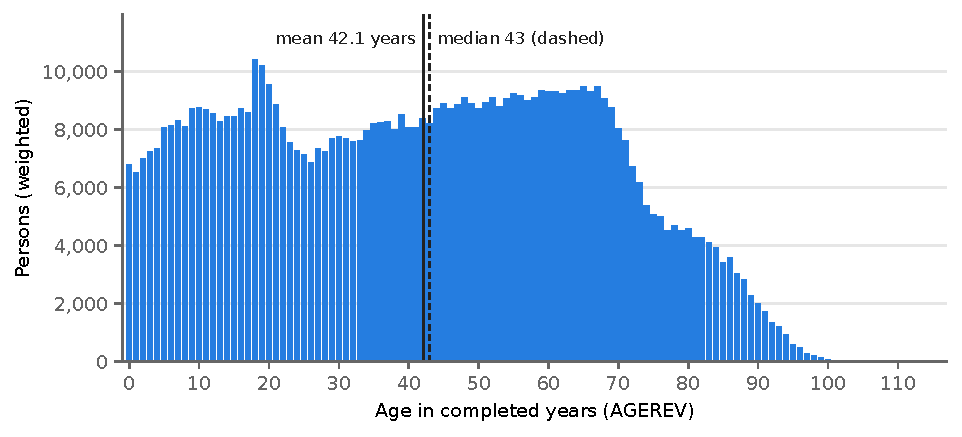
\includegraphics[width=\textwidth]{age_distribution}
  \caption{Weighted age distribution of the population of Calvados (persons per single year of age, \code{AGEREV}),
  with the weighted mean (solid) and median (dashed). Data: INSEE RP2019 detailed census~\cite{insee-census-detailed},
  weights \code{IPONDI}.}
  \label{fig:age-distribution}
\end{figure}

\paragraph{Result.}
The \textbf{average age of the persons living in Calvados is 42.1 years} (weighted mean of \code{AGEREV}); the median is
43 years. With \code{AGED} the mean would be 43.0 years, about one year more, because \code{AGED} counts the birthday of
the census year in advance. \Cref{fig:age-distribution} shows a sharp peak at 18--19 years, a trough in the mid-twenties
(minimum at 26 years), and a broad plateau from about 45 to 68 years (the baby-boom cohorts), followed by a steep
decline after 70. The peak at 18--19 reflects young people who come to study in Caen; the trough means that many of
them leave again after their studies. 21.5\,\% of the population is 65 or older and 23.8\,\% is younger than 20.
Without weights the mean age would be 41.2 years, 0.8 years too low: observations in the large municipalities, which
are younger (\cref{tab:mean-age-validation}), carry smaller weights (\cref{tab:study-area-weights}) and are therefore
over-represented among the rows.

\subsection{Average age per municipality, youngest and oldest (1 point)}

\paragraph{Method.}
Because the detailed file identifies only 17 municipalities (37.7\,\% of the population, \cref{sec:study-area}), a
map of all 528 municipalities cannot be built from it. The average age per municipality is therefore estimated from
the ten age bands of the aggregated census (0--2, 3--5, 6--10, 11--17, 18--24, 25--39, 40--54, 55--64, 65--79 and
80 years or more). Every person of a band $b$ is given the band midpoint $m_b = (l_b + u_b)/2$ in completed years
(e.g.\ 32 for 25--39). For the open band 80+ we assume $m_b = 85$ years; in the detailed file the actual weighted mean
age of this band is 85.7 years. The estimate for municipality $i$ is
$\hat a_i = \sum_b m_b P_{ib} / \sum_b P_{ib}$, where $P_{ib}$ is the population of $i$ in band $b$ and
$\sum_b P_{ib}$ equals \code{P19\_POP}.

\paragraph{Validation.}
For the department and the 17 identifiable municipalities we compare the exact weighted mean age from single-year
ages with the band estimate applied to the same persons of the detailed file (\cref{tab:mean-age-validation}). The
difference is the error of the band approximation alone: 0.08 years for the department, between $-0.16$ and $+0.28$
years for the municipalities (mean $+0.08$). The band estimate from the aggregated file is also shown. It adds the
difference between the two exploitations of the census and deviates by up to 1.1 years (Colombelles), but it ranks
the 17 municipalities almost identically (Spearman correlation 0.99). The approximation is therefore accurate enough
to compare municipalities.

\begin{table}[H]
  \centering
  \caption{Mean age (years): exact weighted mean from single-year ages vs.\ band-midpoint estimate, for the department
  and the 17 municipalities identifiable in the detailed census, sorted by exact mean age. Error = estimate $-$ exact.}
  \label{tab:mean-age-validation}
  \small
  \begin{tabular}{@{}lrrrrr@{}}
    \toprule
    & \multicolumn{3}{c}{Detailed census} & \multicolumn{2}{c}{Aggregated census} \\
    \cmidrule(lr){2-4}\cmidrule(l){5-6}
    Area & Exact & Bands & Error & Bands & Error \\
    \midrule
    \textbf{Calvados (department)} & \textbf{42.05} & \textbf{42.13} & \textbf{+0.08} & \textbf{42.06} & \textbf{+0.01} \\
    \midrule
    H\'erouville-Saint-Clair & 37.85 & 38.13 & +0.28 & 38.11 & +0.26 \\
    Caen & 38.72 & 38.98 & +0.25 & 38.99 & +0.27 \\
    Ifs & 39.23 & 39.40 & +0.18 & 39.38 & +0.15 \\
    Fleury-sur-Orne & 40.66 & 40.79 & +0.13 & 40.96 & +0.30 \\
    Colombelles & 41.18 & 41.41 & +0.23 & 40.09 & $-$1.09 \\
    Giberville & 41.65 & 41.59 & $-$0.06 & 41.49 & $-$0.15 \\
    Mondeville & 42.64 & 42.89 & +0.25 & 42.51 & $-$0.13 \\
    Honfleur & 43.15 & 43.21 & +0.06 & 43.47 & +0.32 \\
    Falaise & 43.46 & 43.32 & $-$0.14 & 43.75 & +0.29 \\
    Lisieux & 43.49 & 43.50 & +0.01 & 43.51 & +0.03 \\
    Cormelles-le-Royal & 44.81 & 45.00 & +0.20 & 44.20 & $-$0.61 \\
    Dives-sur-Mer & 45.66 & 45.66 & +0.00 & 46.12 & +0.46 \\
    Cond\'e-en-Normandie & 45.76 & 45.83 & +0.07 & 45.87 & +0.11 \\
    Vire Normandie & 46.53 & 46.59 & +0.06 & 46.55 & +0.02 \\
    Bayeux & 47.09 & 47.18 & +0.09 & 47.16 & +0.07 \\
    Ouistreham & 50.67 & 50.51 & $-$0.16 & 49.97 & $-$0.69 \\
    Trouville-sur-Mer & 52.39 & 52.27 & $-$0.12 & 52.02 & $-$0.37 \\
    \bottomrule
  \end{tabular}
\end{table}

\begin{figure}[H]
  \centering
  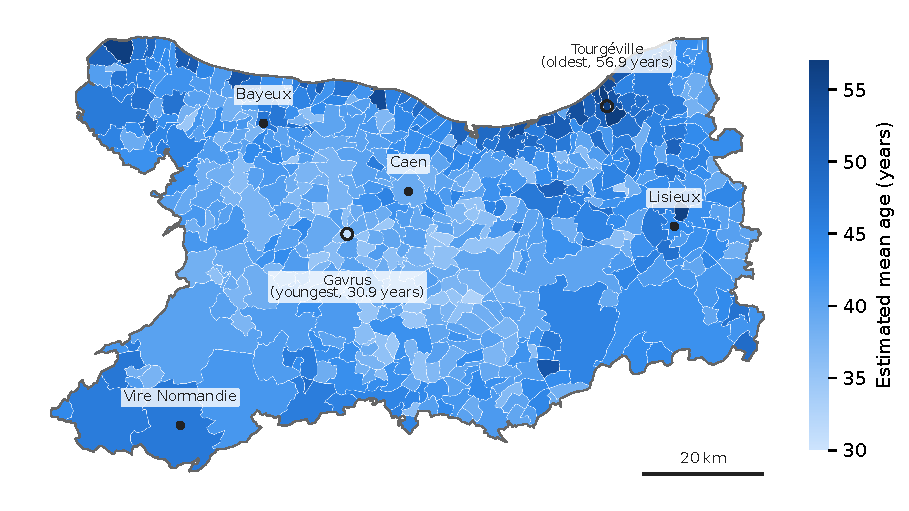
\includegraphics[width=\textwidth]{mean_age_map}
  \caption{Estimated mean age (years) of the population of the 528 municipalities of Calvados, from the age bands of
  the aggregated census RP2019 (band midpoints, 80+ set to 85 years). Circles: youngest and oldest municipality with at
  least 500 inhabitants. Data: INSEE~\cite{insee-census-aggregated}, IGN CONTOURS-IRIS 2021~\cite{ign-contours-iris};
  Lambert-93.}
  \label{fig:mean-age-map}
\end{figure}

\paragraph{Result.}
The estimated mean age of the municipalities ranges from 30.9 to 56.9 years (median 41.4). We name the youngest and the
oldest municipality (a)~over all 528 municipalities and (b)~over the 242 municipalities with at least 500 inhabitants
(90.2\,\% of the population), because the mean age of a municipality of a few dozen inhabitants depends on a handful
of households (\cref{tab:youngest-oldest}). Both variants give the same answer:
\begin{itemize}
  \item \textbf{Youngest: Gavrus} (14297), 584 inhabitants, estimated mean age 30.9 years;
  \item \textbf{Oldest: Tourg\'eville} (14701), 782 inhabitants, estimated mean age 56.9 years.
\end{itemize}
The threshold changes the rest of the ranking: without it, very small municipalities such as Soignolles (128
inhabitants) and Le Fournet (71) appear among the youngest, and Rocques (289) among the oldest.

\begin{table}[H]
  \centering
  \caption{The five youngest and five oldest municipalities by estimated mean age (aggregated census RP2019),
  (a)~all municipalities and (b)~municipalities with at least 500 inhabitants. Population: \code{P19\_POP}.}
  \label{tab:youngest-oldest}
  \small
  \begin{tabular}{@{}llrr@{\hspace{2em}}llrr@{}}
    \toprule
    \multicolumn{4}{c}{(a) All 528 municipalities} & \multicolumn{4}{c}{(b) $\geq$ 500 inhabitants (242)} \\
    \cmidrule(r{2em}){1-4}\cmidrule{5-8}
    Code & Municipality & Pop. & Age & Code & Municipality & Pop. & Age \\
    \midrule
    \multicolumn{8}{@{}l}{\emph{Youngest}} \\
    14297 & Gavrus & 584 & 30.9 & 14297 & Gavrus & 584 & 30.9 \\
    14674 & Soignolles & 128 & 32.8 & 14092 & Bourgu\'ebus & 2{,}186 & 34.2 \\
    14285 & Le Fournet & 71 & 33.6 & 14396 & Maltot & 1{,}024 & 34.6 \\
    14092 & Bourgu\'ebus & 2{,}186 & 34.2 & 14039 & Barbery & 824 & 34.9 \\
    14082 & La Boissi\`ere & 189 & 34.5 & 14207 & Croisilles & 646 & 35.1 \\
    \midrule
    \multicolumn{8}{@{}l}{\emph{Oldest}} \\
    14220 & Deauville & 3{,}565 & 54.6 & 14754 & Villers-sur-Mer & 2{,}543 & 53.9 \\
    14191 & Courseulles-sur-Mer & 4{,}196 & 54.8 & 14220 & Deauville & 3{,}565 & 54.6 \\
    14540 & Rocques & 289 & 56.3 & 14191 & Courseulles-sur-Mer & 4{,}196 & 54.8 \\
    14312 & Grandcamp-Maisy & 1{,}536 & 56.8 & 14312 & Grandcamp-Maisy & 1{,}536 & 56.8 \\
    14701 & Tourg\'eville & 782 & 56.9 & 14701 & Tourg\'eville & 782 & 56.9 \\
    \bottomrule
  \end{tabular}
\end{table}

\Cref{fig:mean-age-map} shows a clear spatial pattern. The oldest municipalities lie on the coast: the seaside resorts
of the C\^ote Fleurie (Tourg\'eville, Deauville, Villers-sur-Mer, Trouville-sur-Mer) and of the C\^ote de Nacre and the
Bessin (Courseulles-sur-Mer, Grandcamp-Maisy), which attract retirees. The youngest are the peri-urban municipalities
around Caen (Gavrus, Maltot, Bourgu\'ebus, Barbery and Croisilles, the light ring south of the city on the map), where
families with children settle. Caen itself and H\'erouville-Saint-Clair are also young (mean ages of 39.0 and 38.1
years in the aggregated file), because of their students and young working population.

\subsection{Socio-professional categories: study area and at least three municipalities (1 point)}

\paragraph{Method.}
All shares refer to the \textbf{population aged 15 and over}, so that the department and the municipalities are
comparable. The SPC counts of the aggregated census are only given for persons aged 15+, and in the detailed file
persons under 15 carry \code{CS1 = 8} (``autres personnes sans activit\'e professionnelle''); without the filter all
children would be counted in category~8. For the \emph{department} we compute the weighted shares of the eight SPCs
from the detailed file (\code{AGEREV} $\geq 15$, weights \code{IPONDI}); the same shares from the aggregated file agree
to within $10^{-14}$ percentage points, as expected since both come from the same exploitation. For the
\emph{municipalities} we use the aggregated file, so that all four areas come from the same source. We chose four
municipalities with contrasting profiles:
\begin{itemize}
  \item \textbf{Caen} (14118, 106{,}230 inhabitants): the main city, regional capital and university town;
  \item \textbf{H\'erouville-Saint-Clair} (14327, 22{,}555): the largest suburb of Caen;
  \item \textbf{Trouville-sur-Mer} (14715, 4{,}603): a seaside resort on the C\^ote Fleurie;
  \item \textbf{\'Epaney} (14240, 511): a rural municipality, chosen by a rule: among the 138 municipalities with
  500 to 1{,}500 inhabitants, the one with the highest share of farmers.
\end{itemize}
The first three are also identifiable in the detailed file, and their weighted shares there are identical to the
aggregated ones. \Cref{fig:spc-distribution} and \cref{tab:spc-shares} compare the shares with the department.

\begin{figure}[H]
  \centering
  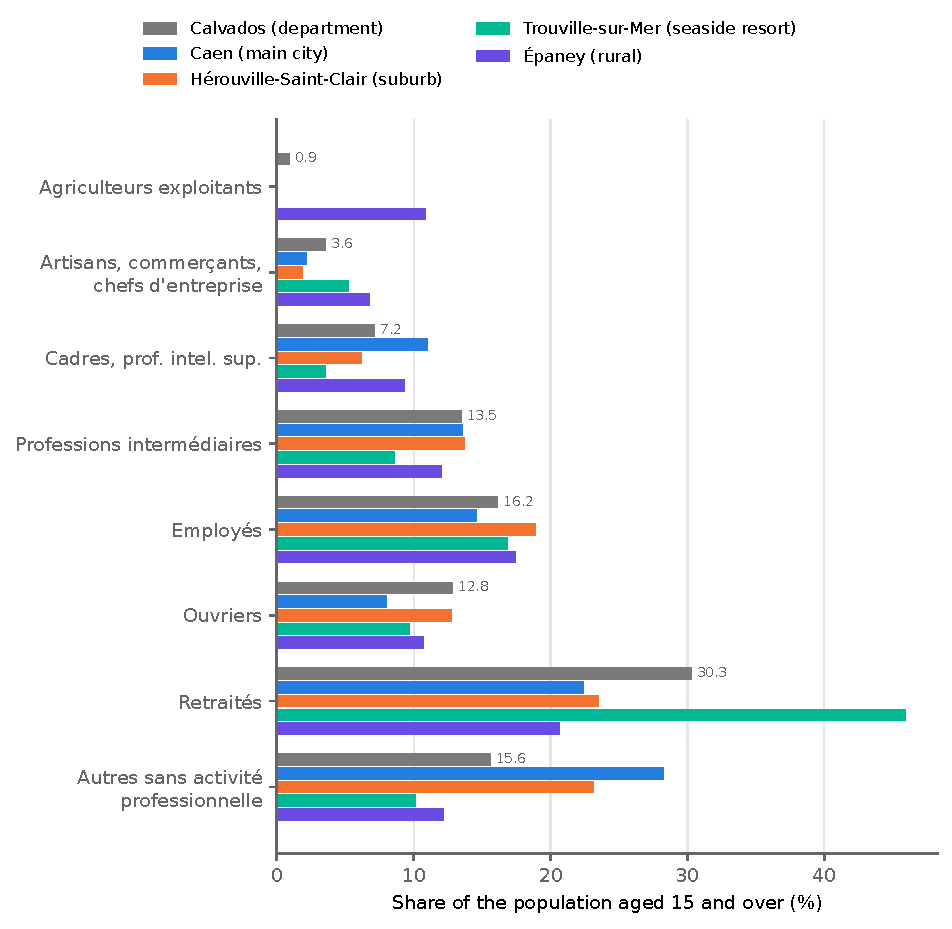
\includegraphics[width=0.9\textwidth]{spc_distribution}
  \caption{Socio-professional categories of the population aged 15 and over: Calvados (grey, reference, value
  labelled) and four municipalities. Shares in \%. Data: INSEE RP2019, aggregated census by
  IRIS~\cite{insee-census-aggregated} (department: identical shares in the weighted detailed
  census~\cite{insee-census-detailed}).}
  \label{fig:spc-distribution}
\end{figure}

\begin{table}[H]
  \centering
  \caption{Socio-professional categories of the population aged 15 and over (\%), Calvados and the four selected
  municipalities (aggregated census RP2019, \code{C19\_POP15P\_CS1} \dots\ \code{CS8}).}
  \label{tab:spc-shares}
  \small
  \begin{tabular}{@{}lrrrrr@{}}
    \toprule
    SPC & Calvados & Caen & H\'erouville & Trouville & \'Epaney \\
    \midrule
    1 Agriculteurs exploitants & 0.9 & 0.1 & 0.0 & 0.0 & 10.9 \\
    2 Artisans, commer\c{c}ants, chefs d'entreprise & 3.6 & 2.1 & 1.8 & 5.3 & 6.8 \\
    3 Cadres, professions intellectuelles sup. & 7.2 & 11.0 & 6.2 & 3.5 & 9.4 \\
    4 Professions interm\'ediaires & 13.5 & 13.5 & 13.7 & 8.6 & 12.0 \\
    5 Employ\'es & 16.2 & 14.6 & 18.9 & 16.9 & 17.4 \\
    6 Ouvriers & 12.8 & 8.0 & 12.7 & 9.7 & 10.7 \\
    7 Retrait\'es & 30.3 & 22.4 & 23.5 & 46.0 & 20.6 \\
    8 Autres sans activit\'e professionnelle & 15.6 & 28.2 & 23.1 & 10.1 & 12.2 \\
    \midrule
    Population 15+ & 576{,}234 & 92{,}552 & 18{,}560 & 4{,}076 & 370 \\
    \bottomrule
  \end{tabular}
\end{table}

\paragraph{Result.}
In the department as a whole, retirees are the largest group (30.3\,\%), followed by employ\'es (16.2\,\%), other
persons without professional activity (15.6\,\%), professions interm\'ediaires (13.5\,\%) and ouvriers (12.8\,\%);
farmers are 0.9\,\%. The municipalities differ clearly from this profile:
\begin{itemize}
  \item \textbf{Caen} has almost twice the department share of persons without professional activity (28.2 vs.\
  15.6\,\%), mostly students, more cadres (11.0 vs.\ 7.2\,\%), and fewer retirees (22.4 vs.\ 30.3\,\%) and ouvriers
  (8.0 vs.\ 12.8\,\%).
  \item \textbf{H\'erouville-Saint-Clair} shares the young profile of Caen (23.1\,\% without activity, 23.5\,\%
  retirees) but has more employ\'es (18.9\,\%) and fewer cadres (6.2\,\%) than both Caen and the department.
  \item \textbf{Trouville-sur-Mer} is dominated by retirees (46.0\,\%, 15.7 percentage points above the department);
  professions interm\'ediaires (8.6\,\%) and cadres (3.5\,\%) are well below the average, artisans and shopkeepers
  slightly above (5.3\,\%).
  \item \textbf{\'Epaney} has twelve times the department share of farmers (10.9 vs.\ 0.9\,\%), more artisans
  (6.8\,\%) and fewer retirees (20.6\,\%). Its shares rest on only 370 persons aged 15+ and are therefore less certain
  than those of the larger municipalities.
\end{itemize}
The SPC profiles match the age pattern of \cref{fig:mean-age-map}: the young urban municipalities have many students and
few retirees, the old coastal resort the reverse.

\paragraph{Problems encountered.}
\begin{itemize}
  \item \emph{Municipalities not identifiable in the detailed census.} Only 17 of 528 municipalities can be identified
  (\cref{sec:study-area}), so the map and the youngest and oldest municipality had to be computed from the aggregated
  census by IRIS. That file has only age bands, so the mean age per municipality is an estimate (band midpoints, 80+
  set to 85 years). We validated it on the 17 identifiable municipalities (\cref{tab:mean-age-validation}).
  \item \emph{Two age variables.} The detailed file has two single-year ages: \code{AGED}, the age reached during the
  census year, and \code{AGEREV}, the age in completed years. \code{AGED} is on average about one year higher. We use
  \code{AGEREV}: it is the usual meaning of age, and only with it do the weighted band totals of the detailed file match
  the age bands of the aggregated file (within 1.0\,\%, against up to 33\,\% with \code{AGED}). The shared census
  file of the project (\code{census\_14.parquet}, written in Exercise~1.1) therefore stores \code{AGEREV} as its
  age column; \code{AGED} is kept only for this comparison.
  \item \emph{Two exploitations of the census.} The population of the aggregated file (\code{P19\_POP},
  \emph{exploitation principale}) and the weights of the detailed file (\emph{exploitation compl\'ementaire}) differ
  slightly, by 0.03\,\% for the department and by up to about one year of mean age for single municipalities
  (Colombelles). The SPC counts of both files come from the same exploitation and agree exactly.
  \item \emph{SPC of children.} Persons under 15 carry \code{CS1 = 8}; all SPC shares therefore use the population 15+.
  A few observations aged 14 in completed years carry another SPC (they turn 15 in the census year). With
  \code{AGEREV} $\geq 15$ the detailed file reproduces the aggregated population 15+ exactly.
  \item \emph{Small municipalities.} Mean ages and SPC shares of very small municipalities rest on few persons. We
  therefore also report the youngest and oldest municipality among municipalities with at least 500 inhabitants and
  chose a rural example with at least 500 inhabitants.
\end{itemize}

\section{Territorial analysis II (Exercise 1.3)}\label{sec:territorial-II}

\paragraph{Data.}
\begin{itemize}
  \item Working inhabitants: aggregated census by IRIS RP2019~\cite{insee-census-aggregated},
  \url{https://www.insee.fr/fr/statistiques/6543200}, already aggregated to the 528 municipalities in
  \cref{sec:territorial-I}.
  \item Employees: URSSAF open data on private-sector employers and salaried employees per municipality and activity
  sector (APE)~\cite{urssaf-employment},\newline
  \href{https://open.urssaf.fr/explore/dataset/etablissements-et-effectifs-salaries-au-niveau-commune-x-ape-last/information/}{\texttt{open.urssaf.fr/explore/dataset/}\newline
  \texttt{etablissements-et-effectifs-salaries-au-niveau-commune-x-ape-last}},
  latest edition (dataset last modified on 29 May 2026, years 2006--2025), CSV export restricted to department 14,
  downloaded on 27 November 2026. We use the column \code{Effectifs salari\'es 2019}, the employees at
  \textbf{31 December 2019}: 2019 is the year of the census RP2019, so that both sources describe the same year, and it
  is also the year used in the course notebook.
  \item INSEE Code officiel g\'eographique 2026, list of changes of municipalities~\cite{insee-cog-2026},
  \url{https://www.insee.fr/fr/statistiques/fichier/8740222/v_mvt_commune_2026.csv}, to recode URSSAF to the 2021
  geography.
  \item For validation only: INSEE commuting file MOBPRO RP2019~\cite{insee-mobpro-2019},
  \url{https://www.insee.fr/fr/statistiques/6456056} (\code{FD\_MOBPRO\_2019.csv}).
\end{itemize}

\subsection{Working inhabitants per municipality (1 point)}

\begin{qa}{Make use of the aggregated census data to create a bar plot indicating the number of working inhabitants in
each municipality of the study area. Explain how you count these persons from the data.}
The bar plot is \cref{fig:working-inhabitants} (30 largest municipalities) and \cref{fig:working-inhabitants-all} in
the appendix (all 528). \textbf{We count as working inhabitants the persons aged 15 and over in the six SPCs of the
working population}, i.e.\ the sum of the columns \code{C19\_POP15P\_CS1} to \code{C19\_POP15P\_CS6} of the
aggregated census, summed from IRIS to municipality. Retirees (SPC~7) and other persons without professional activity
(SPC~8) are excluded. Calvados has 311{,}886 working inhabitants; Caen has the most (45{,}682).
\end{qa}

\paragraph{Method.}
The aggregated census does not count employed persons directly. It gives the population aged 15 and over in eight
socio-professional categories (SPC). As in the trip production model of \cref{sec:trip-production}, the
\emph{working inhabitants} of municipality $i$ are the persons aged 15 and over in the six SPCs of the working
population:
\begin{equation*}
  W^{\mathrm{res}}_i = \code{C19\_POP15P\_CS1} + \code{C19\_POP15P\_CS2} + \dots + \code{C19\_POP15P\_CS6},
\end{equation*}
i.e.\ agriculteurs exploitants; artisans, commer\c{c}ants and chefs d'entreprise; cadres and professions
intellectuelles sup\'erieures; professions interm\'ediaires; employ\'es; and ouvriers. SPC~7 (retrait\'es) and SPC~8
(autres personnes sans activit\'e professionnelle, mostly pupils, students and persons at home) are excluded. The
values per IRIS are summed to municipalities. They are weighted counts from the \emph{exploitation compl\'ementaire}
of the census, so they are not integers.
\begin{lstlisting}[style=py]
WORKING_SPC = [1, 2, 3, 4, 5, 6]        # 7 (retraites) and 8 (autres) excluded
WORKING_COLUMNS = [f"C19_POP15P_CS{k}" for k in WORKING_SPC]
df_population["working_inhabitants"] = df_population[WORKING_COLUMNS].sum(axis=1)
\end{lstlisting}

The SPC classifies persons by ``la profession (ou l'ancienne profession)''~\cite{insee-rp-definitions}. SPC 1--6
therefore count the \emph{active} population by occupation, which may include persons who are not in employment. We
measured this in the detailed census, which comes from the same exploitation as the SPC counts. We cross-tabulated
SPC and activity status (\code{TACT}) for the persons aged 15 and over of the department, with weights. Of the persons
in SPC 1--6, \textbf{88.9\,\% are employed and 11.1\,\% unemployed}. No other activity status occurs, and every
employed person is in SPC 1--6. Unemployed persons who never worked are in SPC~8. The department has 277{,}131
employed persons aged 15 and over. We keep the definition above, because the exercise asks for the aggregated census
per municipality, which has no activity status. $W^{\mathrm{res}}_i$ therefore exceeds the employed residents by
12.5\,\% at department level, and the unemployed share differs between municipalities. This difference is small
compared with the gap between the census and URSSAF, which covers only 58\,\% of the working inhabitants
(\cref{sec:territorial-II-difference}).

\begin{figure}[H]
  \centering
  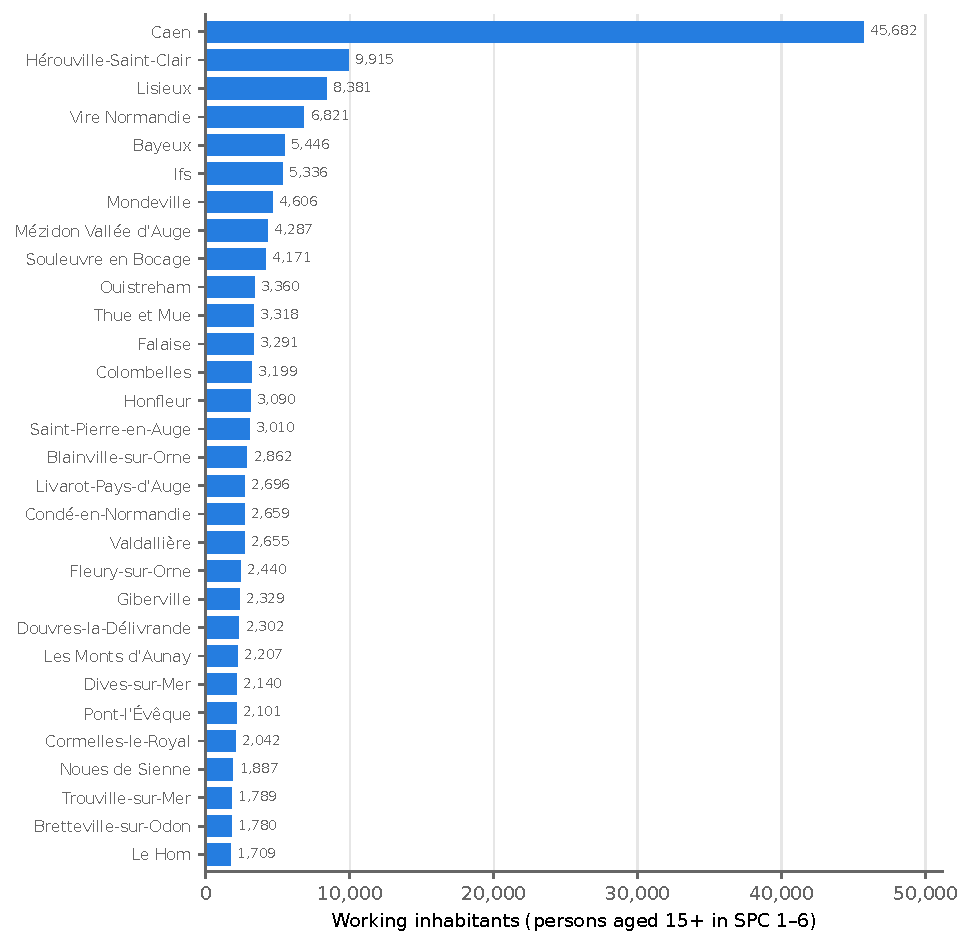
\includegraphics[width=0.85\textwidth]{working_inhabitants_top30}
  \caption{Working inhabitants (persons aged 15 and over in SPC 1--6) of the 30 municipalities of Calvados with the
  most working inhabitants. All 528 municipalities: \cref{fig:working-inhabitants-all} in the appendix. Data:
  INSEE RP2019, aggregated census by IRIS~\cite{insee-census-aggregated}.}
  \label{fig:working-inhabitants}
\end{figure}

\paragraph{Result.}
Calvados has \textbf{311{,}886 working inhabitants}: 54.1\,\% of the 576{,}234 persons aged 15 and over and 44.9\,\%
of the population. The weighted count of persons aged 15+ with SPC 1--6 in the detailed census gives the same total,
because both come from the same exploitation. \Cref{fig:working-inhabitants} shows the 30 largest municipalities.
Caen dominates with 45{,}682 working inhabitants (14.6\,\% of the department), followed by its suburb
H\'erouville-Saint-Clair (9{,}915) and the three other towns Lisieux (8{,}381), Vire Normandie (6{,}821) and Bayeux
(5{,}446). The top 30 municipalities hold 47.3\,\% of all working inhabitants. The median municipality has only 202
working inhabitants, and the smallest (Rapilly) has 10. A bar plot of all 528 municipalities, sorted, is in the
appendix (\cref{fig:working-inhabitants-all}).

\subsection{Employees per municipality (1 point)}

\begin{qa}{Make use of the URSSAF employment data to create a bar plot indicating the number of employees in each
municipality of the study area.}
The bar plot is \cref{fig:employees} (30 largest municipalities) and \cref{fig:employees-all} in the appendix
(all 528). URSSAF counts \textbf{180{,}618 private-sector salaried employees} in Calvados in 2019; Caen has the most
(35{,}246), followed by Mondeville (10{,}500).
\end{qa}

\paragraph{Method.}
The URSSAF file has one row per municipality and APE code with the number of establishments and of salaried employees
at 31 December of each year. As in the course notebook, we read \code{Code commune} as a string, keep the department
(CSV export with the filter \code{code\_departement:14}: 16{,}301 rows), and sum \code{Effectifs salari\'es 2019} over
all APE codes. Empty values are counted as 0. Of the 7{,}480 empty values, 7{,}476 belong to sectors without any
establishment in the municipality in 2019, and 4 to rows with one establishment but no count.

URSSAF uses the current geography of municipalities, while the project uses the 528 municipalities of 2021. The changes
since 1 January 2021 are taken from the INSEE list of changes of municipalities~\cite{insee-cog-2026}. Three of our
municipalities are affected:
\begin{itemize}
  \item Aurseulles changed its code from 14011 to 14581 (24 April 2024, new chef-lieu). We relabel it.
  \item Saint-Martin-de-Fontenay (14623) merged with May-sur-Orne (14408) into Saint-Martin-de-May (14408) on 1 January
  2025, with 406 employees in 2019.
  \item Gerrots (14300) merged into Victot-en-Auge (14743) on 1 January 2025, with 12 employees in 2019.
\end{itemize}
URSSAF reports only the totals of the merged municipalities. We split each total between the 2021 municipalities in
proportion to their working inhabitants. This is an assumption, and the split affects 418 employees. After recoding,
every URSSAF row is matched, and the department total is preserved. Ten small municipalities (48 to 216 inhabitants)
have no URSSAF row at all. They get \textbf{0 employees}, which means no private establishment with employees. In
total, 55 municipalities have 0 employees in 2019.
\begin{lstlisting}[style=py]
# Sum over all APE sectors per municipality (empty values count as 0)
df_urssaf = (df_urssaf_raw.groupby("Code commune")
             .agg(employees=("Effectifs salariés 2019", "sum"))
             .rename_axis("urssaf_code").reset_index())

# 2021 code -> current code, following the INSEE list of changes after 1 January 2021
changes = df_cog[
    (df_cog["DATE_EFF"] > "2021-01-01") & (df_cog["TYPECOM_AV"] == "COM") & (df_cog["TYPECOM_AP"] == "COM")
    & df_cog["COM_AV"].isin(ours) & (df_cog["COM_AV"] != df_cog["COM_AP"])
]
to_current = dict(zip(changes["COM_AV"], changes["COM_AP"]))
def current_code(code):
    while code in to_current:
        code = to_current[code]
    return code
df_match["urssaf_code"] = df_match["municipality_id"].map(current_code)

# Split the total of a merged municipality in proportion to the working inhabitants
df_match = df_match.merge(df_urssaf, on="urssaf_code", how="left", validate="m:1")
group_working = df_match.groupby("urssaf_code")["working_inhabitants"].transform("sum")
df_match["n_in_group"] = df_match.groupby("urssaf_code")["municipality_id"].transform("size")
df_match["split_share"] = np.where(df_match["n_in_group"] > 1,
                                   df_match["working_inhabitants"] / group_working, 1.0)
df_match["employees"] = (df_match["employees"] * df_match["split_share"]).fillna(0.0)   # no row -> 0
\end{lstlisting}

\emph{Scope.} URSSAF counts \emph{private-sector salaried employees at their place of work}. Not included are the
public sector (State, local authorities, public hospitals), the self-employed, and farmers and agricultural employees,
who are covered by the MSA.

\begin{figure}[H]
  \centering
  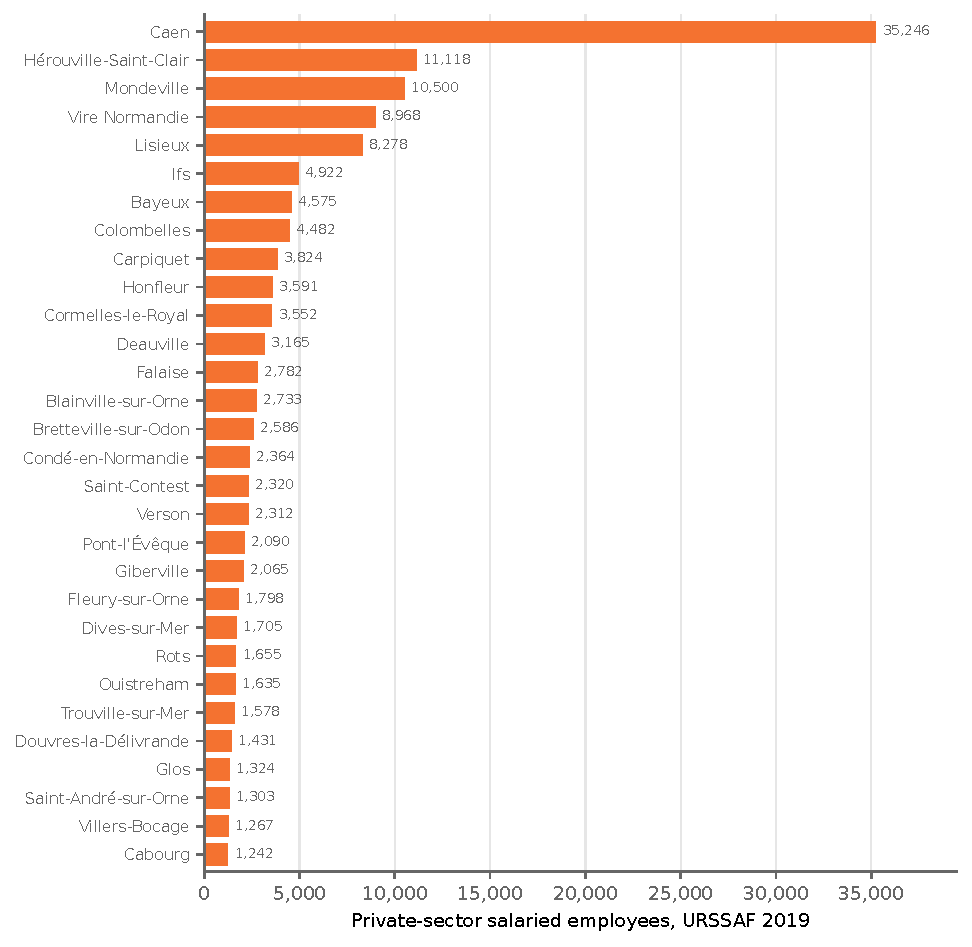
\includegraphics[width=0.85\textwidth]{employees_top30}
  \caption{Private-sector salaried employees at 31 December 2019 of the 30 municipalities of Calvados with the most
  employees, summed over all APE codes. All 528 municipalities: \cref{fig:employees-all} in the appendix. Data:
  URSSAF~\cite{urssaf-employment}.}
  \label{fig:employees}
\end{figure}

\paragraph{Result.}
URSSAF counts \textbf{180{,}618 private-sector salaried employees in Calvados in 2019}. Employment is much more
concentrated than residence (\cref{fig:employees}). Caen has 35{,}246 employees (19.5\,\% of the department), and the
top 30 municipalities hold 75.5\,\% of all employees, against 47.3\,\% of the working inhabitants. The median
municipality has 16 employees. Next to the towns, the list contains employment zones around Caen that are small as
places of residence: Mondeville (10{,}500 employees, third), Carpiquet (airport, 3{,}824), Saint-Contest, Verson and
Rots.

\subsection{Difference between working inhabitants and employees (1 point)}\label{sec:territorial-II-difference}

\begin{qa}{Make a map of the study area which, for each municipality, shows the difference between working inhabitants
and employees. Which municipality has the largest net outflow (inhabitants $-$ employees), which one the largest net
inflow of employees?}
The map is \cref{fig:net-flow-map}. \textbf{The answer to the question as asked}, i.e.\ for the raw difference
working inhabitants $-$ employees, is: the \textbf{largest net outflow is Caen} (14118, $+10{,}436$) and the
\textbf{largest net inflow is Mondeville} (14437, $-5{,}894$).

As an additional reading, we also scale the employees to the total of working inhabitants
(\cref{fig:net-flow-map-scaled}). Caen's raw outflow is an artefact of URSSAF, which misses the public-sector jobs
concentrated there, so the scaled view is more meaningful and is confirmed by the commuting data MOBPRO. In it the
largest net outflow is Souleuvre en Bocage (14061, $+3{,}032$) and the largest net inflow is Caen ($-15{,}179$).
\end{qa}

\paragraph{Method.}
For each municipality we compute $\Delta_i = W^{\mathrm{res}}_i - E_i$, working inhabitants minus employees. A
positive value means more working residents than jobs, i.e.\ a \emph{net outflow} of commuters. A negative value means
a \emph{net inflow} of employees. The map (\cref{fig:net-flow-map}) uses a diverging colour scale centred at 0, with
blue for inflow and red for outflow, and symmetric limits $\pm\max_i|\Delta_i|$. Caen alone reaches $\pm 10^4$, so
the scale is a symmetric logarithm: linear within $\pm 100$ persons and logarithmic beyond.

\paragraph{Comparability.}
The two sources do not measure the same thing. The census counts all working residents, at their place of residence:
the public sector, the self-employed and farmers, and unemployed persons with a former occupation (11.1\,\% of SPC
1--6). URSSAF counts private salaried jobs, at the place of work. The totals are 311{,}886 working inhabitants and 180{,}618
employees: URSSAF covers only \textbf{58\,\%} of the census count (ratio 0.579). The raw difference is therefore
positive in 505 of the 528 municipalities and sums to $+131{,}268$. As an additional view, we scale the employees to
the total of working inhabitants, $\tilde E_i = E_i \cdot \sum_k W^{\mathrm{res}}_k / \sum_k E_k$ (factor 1.727). The
scaled difference $\tilde\Delta_i = W^{\mathrm{res}}_i - \tilde E_i$ sums to 0 and shows the relative pattern
(\cref{fig:net-flow-map-scaled}). This is also how employment enters the trip attraction in \cref{sec:trip-attraction}:
arriving trips are proportional to employment.
\begin{lstlisting}[style=py]
df_population["difference"] = df_population["working_inhabitants"] - df_population["employees"]
scale_factor = working_total / employees_total                     # 1.727
df_population["difference_scaled"] = (df_population["working_inhabitants"]
                                      - scale_factor * df_population["employees"])
outflow = df_population.nlargest(1, "difference")     # largest net outflow
inflow = df_population.nsmallest(1, "difference")     # largest net inflow
\end{lstlisting}

\begin{figure}[H]
  \centering
  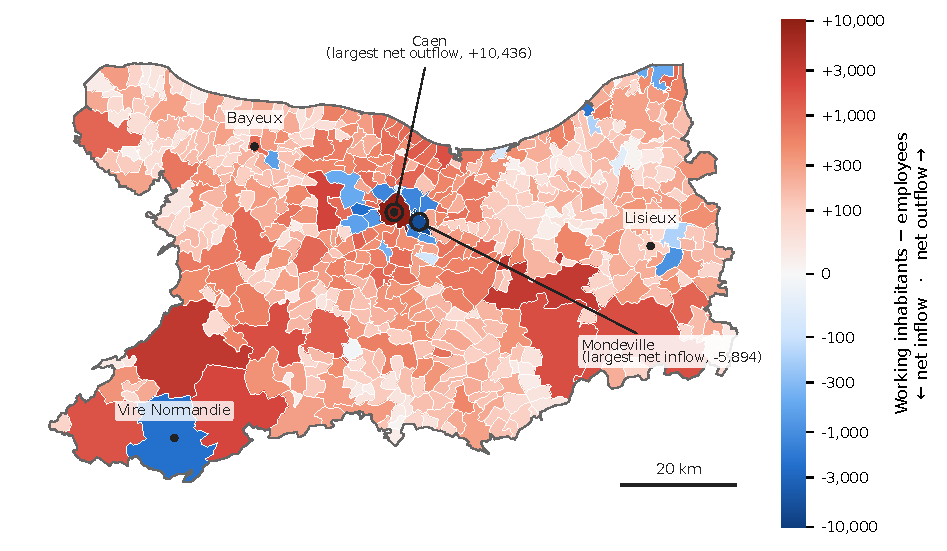
\includegraphics[width=\textwidth]{inhabitants_minus_employees_map}
  \caption{Working inhabitants (census RP2019, SPC 1--6) minus private-sector salaried employees (URSSAF 2019) per
  municipality. Red: net outflow; blue: net inflow. Symmetric logarithmic colour scale, linear within $\pm 100$.
  Circles: largest net outflow and largest net inflow. Data: INSEE~\cite{insee-census-aggregated},
  URSSAF~\cite{urssaf-employment}, IGN CONTOURS-IRIS 2021~\cite{ign-contours-iris}; Lambert-93.}
  \label{fig:net-flow-map}
\end{figure}

\paragraph{Result.}
\begin{itemize}
  \item \textbf{Largest net outflow: Caen} (14118): 45{,}682 working inhabitants, 35{,}246 employees, difference
  $+10{,}436$.
  \item \textbf{Largest net inflow: Mondeville} (14437): 4{,}606 working inhabitants, 10{,}500 employees, difference
  $-5{,}894$.
\end{itemize}
The result for Caen is an effect of the definitions. Caen is the main employment centre of the department, but it
concentrates the public-sector jobs that URSSAF does not count (university, regional hospital, administrations).
Its working residents are therefore compared with its private jobs only. Mondeville, with commercial and industrial zones
east of Caen, has more than twice as many private jobs as working residents.

Only 23 municipalities have a net inflow in the raw view: the employment zones around Caen (Mondeville, Carpiquet,
Cormelles-le-Royal, H\'erouville-Saint-Clair, Colombelles), Vire Normandie, and the resort Deauville
(\cref{tab:net-flow-top5}). The largest outflows are Caen and large rural \emph{communes nouvelles} with few private
jobs (Souleuvre en Bocage, M\'ezidon Vall\'ee d'Auge, Thue et Mue, Valdalli\`ere).

\begin{table}[H]
  \centering
  \caption{The five municipalities with the largest net outflow and the five with the largest net inflow, raw
  difference $\Delta_i$ and scaled difference $\tilde\Delta_i$ (employees $\times\,1.727$). Bold: the answer per view.}
  \label{tab:net-flow-top5}
  \small
  \setlength{\tabcolsep}{4pt}
  \begin{tabular}{@{}llrrr@{\hspace{1.5em}}llr@{}}
    \toprule
    \multicolumn{5}{c}{Raw: $\Delta_i = W^{\mathrm{res}}_i - E_i$} & \multicolumn{3}{c}{Scaled: $\tilde\Delta_i$} \\
    \cmidrule(r{1.5em}){1-5}\cmidrule{6-8}
    Code & Municipality & $W^{\mathrm{res}}_i$ & $E_i$ & $\Delta_i$ & Code & Municipality & $\tilde\Delta_i$ \\
    \midrule
    \multicolumn{8}{@{}l}{\emph{Largest net outflow}} \\
    14118 & \textbf{Caen} & 45{,}682 & 35{,}246 & $+$10{,}436 & 14061 & \textbf{Souleuvre en Bocage} & $+$3{,}032 \\
    14061 & Souleuvre en Bocage & 4{,}171 & 660 & $+$3{,}511 & 14431 & M\'ezidon Vall\'ee d'Auge & $+$2{,}814 \\
    14431 & M\'ezidon Vall\'ee d'Auge & 4{,}287 & 853 & $+$3{,}434 & 14726 & Valdalli\`ere & $+$1{,}805 \\
    14098 & Thue et Mue & 3{,}318 & 907 & $+$2{,}411 & 14098 & Thue et Mue & $+$1{,}752 \\
    14726 & Valdalli\`ere & 2{,}655 & 492 & $+$2{,}163 & 14027 & Les Monts d'Aunay & $+$1{,}561 \\
    \midrule
    \multicolumn{8}{@{}l}{\emph{Largest net inflow}} \\
    14437 & \textbf{Mondeville} & 4{,}606 & 10{,}500 & $-$5{,}894 & 14118 & \textbf{Caen} & $-$15{,}179 \\
    14137 & Carpiquet & 1{,}495 & 3{,}824 & $-$2{,}329 & 14437 & Mondeville & $-$13{,}525 \\
    14762 & Vire Normandie & 6{,}821 & 8{,}968 & $-$2{,}147 & 14327 & H\'erouville-Saint-Clair & $-$9{,}283 \\
    14220 & Deauville & 1{,}283 & 3{,}165 & $-$1{,}882 & 14762 & Vire Normandie & $-$8{,}665 \\
    14181 & Cormelles-le-Royal & 2{,}042 & 3{,}552 & $-$1{,}510 & 14366 & Lisieux & $-$5{,}913 \\
    \bottomrule
  \end{tabular}
\end{table}

\begin{figure}[H]
  \centering
  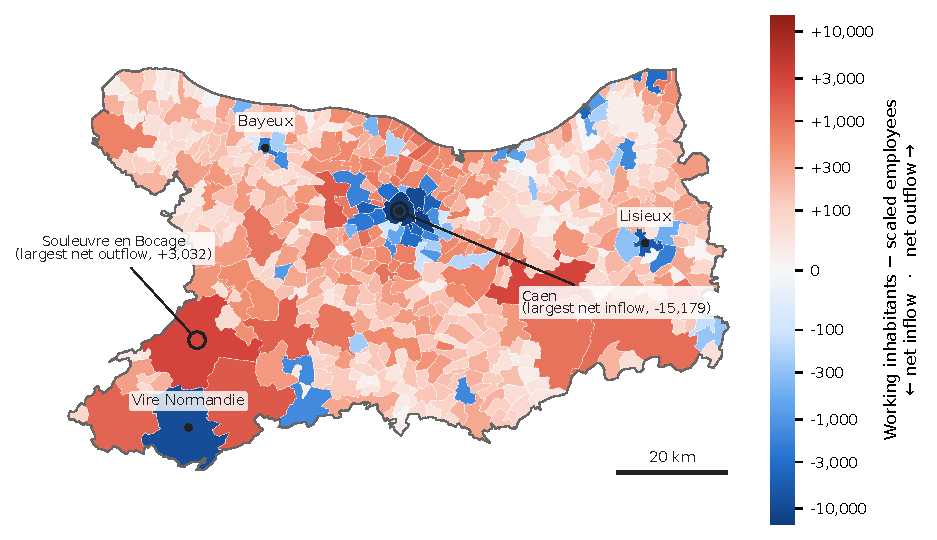
\includegraphics[width=\textwidth]{inhabitants_minus_employees_scaled_map}
  \caption{Working inhabitants minus \emph{scaled} employees, $\tilde\Delta_i = W^{\mathrm{res}}_i - 1.727\,E_i$
  (employees scaled to the total of working inhabitants). Same colour scale as \cref{fig:net-flow-map}, with
  symmetric limits $\pm 15{,}179$. Data as in \cref{fig:net-flow-map}.}
  \label{fig:net-flow-map-scaled}
\end{figure}

\paragraph{Scaled view.}
After scaling, the picture matches the urban structure (\cref{fig:net-flow-map-scaled}). \textbf{Caen becomes the
largest net inflow} ($-15{,}179$), followed by Mondeville, H\'erouville-Saint-Clair, Vire Normandie and Lisieux.
\textbf{The largest net outflow is Souleuvre en Bocage} (14061; $+3{,}032$), a rural commune nouvelle north-east of Vire.
36 municipalities change side, all from outflow to inflow. Together they hold 33.7\,\% of the working inhabitants.
They include Caen, Lisieux, Bayeux, Ifs, Falaise, Condé-en-Normandie and Pont-l'\'Ev\^eque, i.e.\ the towns whose
private employment is close to their number of working residents. The number of inflow municipalities rises from 23
to 59. The scaled view assumes that the jobs URSSAF does not count are distributed like private salaried jobs. It is
not exact either, but it is the more meaningful answer to the question. It is also the assumption used for the
trip attraction in \cref{sec:trip-attraction}.

\subsection{Validation with commuting data}\label{sec:territorial-II-mobpro}

\paragraph{Data.}
INSEE's commuting file MOBPRO~\cite{insee-mobpro-2019} gives, for every employed person of the census RP2019, the
municipality of residence (\code{COMMUNE}) and the municipality of work (\code{DCLT}), with the weight \code{IPONDI}.
Unlike URSSAF, it covers \emph{all} jobs, including the public sector, the self-employed and farmers. It uses the same
year (2019) and the same geography (2021) as our census. It is therefore the real-data reference for the net commuting
balance of each municipality. As in the course notebook, we read \code{COMMUNE}, \code{ARM}, \code{DCLT},
\code{IPONDI} and \code{TRANS} in chunks. We keep every person who lives \emph{or} works in Calvados, so that commuters
from and to other departments are included. All department codes in the file are among our 528 municipalities. Every
municipality has employed residents, and 7 small municipalities have no job. For each municipality $i$ we compute
the employed residents $R_i$ (living in $i$), the jobs $J_i$ (working in $i$, wherever the person lives) and the net
balance $N_i = R_i - J_i$, with the same sign convention as $\Delta_i$. This is a validation only: the answers above
remain those based on the census and URSSAF, as the exercise asks.

\begin{table}[H]
  \centering
  \caption{Department totals of Calvados, 2019. The census counts are at the place of residence, the job counts at
  the place of work. Data: INSEE~\cite{insee-census-aggregated,insee-census-detailed,insee-mobpro-2019},
  URSSAF~\cite{urssaf-employment}.}
  \label{tab:mobpro-totals}
  \begin{tabular}{@{}llr@{}}
    \toprule
    Quantity & Counted at & Persons \\
    \midrule
    Census: working inhabitants $W^{\mathrm{res}}$ (aged 15+, SPC 1--6) & residence & 311{,}886 \\
    Census: employed persons aged 15+ (\code{TACT} $=$ 11) & residence & 277{,}131 \\
    MOBPRO: employed residents $R$ & residence & 277{,}131 \\
    MOBPRO: jobs located in Calvados $J$ & workplace & 275{,}908 \\
    URSSAF: private-sector salaried employees $E$ & workplace & 180{,}618 \\
    \bottomrule
  \end{tabular}
\end{table}

\paragraph{Totals.}
MOBPRO counts exactly the employed persons of the detailed census (\cref{tab:mobpro-totals}), because both are the
same census records with the same weights. The working inhabitants are 12.5\,\% higher, as measured in
\cref{sec:territorial-II} with \code{TACT}. Per municipality, $W^{\mathrm{res}}_i$ and $R_i$ correlate at 0.9997, and
the median ratio is 1.09. The SPC definition therefore shifts the level but hardly changes the pattern. 30.0\,\% of
the employed residents work in their own municipality. 21{,}882 residents (7.9\,\%) work outside Calvados, mainly in
Manche, Orne, Seine-Maritime, Eure and Paris. 20{,}659 persons living outside work in Calvados, mainly from Manche,
Eure and Orne. Calvados is therefore almost balanced: 1{,}223 more residents commute out than workers commute in.

\paragraph{Jobs not counted by URSSAF.}
URSSAF covers 65.5\,\% of the 275{,}908 jobs located in Calvados. Of the 95{,}290 jobs that URSSAF misses, 40\,\%
are in Caen, which has 73{,}271 jobs but only 35{,}246 URSSAF employees (coverage 48\,\%: university, regional
hospital, administrations). Next come Lisieux (5{,}215 jobs missed), Bayeux (3{,}817), Falaise and Vire Normandie,
towns with hospitals, schools and sub-prefectures. This confirms the explanation given for Caen in
\cref{sec:territorial-II-difference}. In 38 municipalities, URSSAF has \emph{more} employees than MOBPRO has jobs,
mostly commercial and industrial zones around Caen (Mondeville $+666$, Bretteville-sur-Odon $+607$). URSSAF counts job
positions at 31 December: persons with two jobs count twice, and temporary workers count where the agency is. MOBPRO
counts persons at the place of their main job.

\begin{figure}[H]
  \centering
  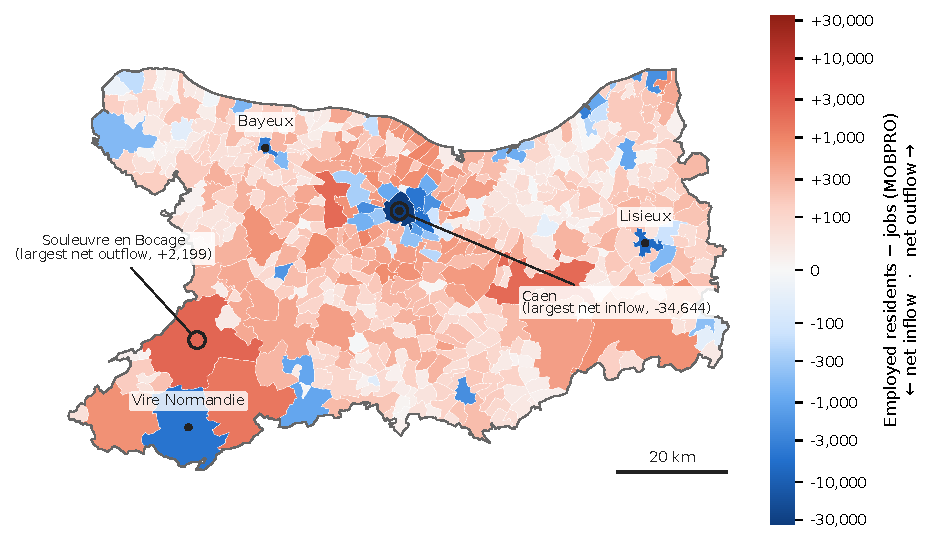
\includegraphics[width=\textwidth]{net_commuting_mobpro_map}
  \caption{Net commuting according to MOBPRO, employed residents minus jobs, per municipality. Red: net outflow;
  blue: net inflow. Same colour scale as \cref{fig:net-flow-map} (symmetric logarithm, linear within $\pm 100$), with
  symmetric limits $\pm 34{,}644$. Data: INSEE MOBPRO RP2019~\cite{insee-mobpro-2019}, IGN CONTOURS-IRIS
  2021~\cite{ign-contours-iris}; Lambert-93.}
  \label{fig:net-commuting-mobpro}
\end{figure}

\begin{figure}[H]
  \centering
  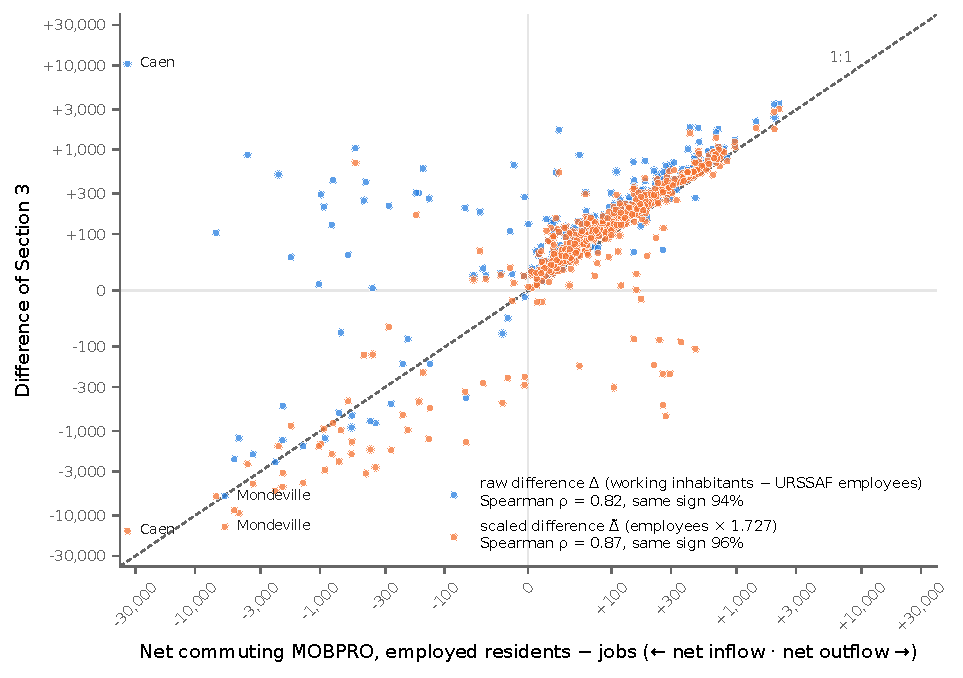
\includegraphics[width=0.9\textwidth]{difference_vs_mobpro}
  \caption{Raw difference $\Delta_i$ (blue) and scaled difference $\tilde\Delta_i$ (orange) of each municipality
  against the net commuting $N_i$ of MOBPRO. Both axes use a symmetric logarithm, linear within $\pm 100$. Points on
  the dashed line agree exactly. Data: as in \cref{fig:net-flow-map,fig:net-commuting-mobpro}.}
  \label{fig:difference-vs-mobpro}
\end{figure}

\paragraph{Net commuting.}
According to MOBPRO (\cref{fig:net-commuting-mobpro}), the \textbf{largest net inflow is Caen} (14118): 38{,}627
employed residents, 73{,}271 jobs, $N = -34{,}644$. Next come Lisieux ($-6{,}749$), Mondeville ($-5{,}785$), Vire
Normandie ($-4{,}837$) and H\'erouville-Saint-Clair ($-4{,}465$). The \textbf{largest net outflow is Souleuvre en
Bocage} (14061; $+2{,}199$), followed by Thue et Mue ($+2{,}020$) and M\'ezidon Vall\'ee d'Auge ($+2{,}009$).
54 municipalities have a net inflow (raw view: 23, scaled view: 59). Both extremes are the answers of the
\emph{scaled} view, while the raw view gives Caen the wrong sign. \Cref{tab:mobpro-agreement} and
\cref{fig:difference-vs-mobpro} show that \textbf{the scaled view is closer to reality} on every measure. Its
magnitudes are still wrong where the mix of jobs is unusual. It finds less than half of Caen's real inflow
($-15{,}179$ against $-34{,}644$) and more than twice the inflow of Mondeville ($-13{,}525$ against $-5{,}785$).
For Mondeville the raw value ($-5{,}894$) is almost exact. Scaling assumes that every municipality has the
department's share of private jobs, which does not hold for an administrative centre or a private employment zone.

\begin{table}[H]
  \centering
  \caption{Agreement of the raw difference $\Delta_i$ and the scaled difference $\tilde\Delta_i$ with the net
  commuting $N_i$ of MOBPRO, over the 528 municipalities.}
  \label{tab:mobpro-agreement}
  \begin{tabular}{@{}lrr@{}}
    \toprule
    Measure & Raw $\Delta_i$ & Scaled $\tilde\Delta_i$ \\
    \midrule
    Pearson correlation & $-0.40$ & 0.78 \\
    Pearson correlation without Caen & 0.68 & 0.90 \\
    Spearman rank correlation & 0.82 & 0.87 \\
    Municipalities with the same sign as $N_i$ & 94.1\,\% & 95.6\,\% \\
    Mean absolute deviation from $N_i$ (persons) & 258 & 208 \\
    \bottomrule
  \end{tabular}
\end{table}

The table of origin--destination flows with both ends in Calvados (255{,}249 persons in 9{,}866 pairs of
municipalities, summed over the modes) is saved for the validation of the gravity model in \cref{sec:trip-distribution}.

\paragraph{Problems encountered.}
\begin{itemize}
  \item \emph{Definition of working inhabitants.} The aggregated census has no count of employed persons, and SPC
  1--6 also classify persons by a former occupation. Measured in the detailed census (SPC $\times$ \code{TACT}),
  88.9\,\% of the persons in SPC 1--6 are employed and 11.1\,\% unemployed, so $W^{\mathrm{res}}_i$ exceeds the
  employed residents by 12.5\,\%. This is small compared with the gap between census and URSSAF: URSSAF counts 58\,\%
  of the working inhabitants and still only 65\,\% of the 277{,}131 employed persons.
  \item \emph{Different municipality geography.} URSSAF uses the current geography, the project that of 2021: one
  change of code (Aurseulles) and two mergers on 1 January 2025 (Saint-Martin-de-Fontenay into Saint-Martin-de-May,
  Gerrots into Victot-en-Auge). Codes were recoded with the INSEE list of changes~\cite{insee-cog-2026}. The merged
  totals (418 employees) were split in proportion to working inhabitants.
  \item \emph{Missing municipalities and empty values.} Ten small municipalities have no URSSAF row and get 0
  employees. The empty 2019 values (7{,}480 rows) are sectors without an establishment in that year and are counted
  as 0.
  \item \emph{Different definitions of the two sources.} Private salaried jobs at the workplace (URSSAF) cover only
  58\,\% of the working residents (census). Without scaling, Caen appears as the largest net outflow, which is an
  effect of the missing public-sector jobs. We therefore report both the raw and the scaled difference.
\end{itemize}

\section{Trip production (Exercise 2.1)}\label{sec:trip-production}
\noindent Responsible: Person A. Notebook: \code{notebooks/A4\_trip\_production\_attraction.ipynb}.

\subsection{Trip generation model and total number of trips (1 point)}

\paragraph{Method.}
The number of originating trips of zone $i$ is obtained from the growth-factor model of the assignment, applied to the
aggregated census \cite{insee-census-aggregated}:
\begin{equation}\label{eq:trip-generation}
  \Oi = \max\!\left(\beta_0 + \sum_{s=1}^{8} \beta_s\, n_{i,s},\; 0\right),
\end{equation}
where $s$ indexes the socio-professional category (SPC), $\beta_s$ is the growth factor of SPC $s$, and $n_{i,s}$ is the
size of the population older than 15 years with SPC $s$ in zone $i$. The offset $\beta_0$ is added \emph{once per
zone}, not once per SPC. The parameters are given in \cref{tab:trip-generation-parameters}. The total number of
generated trips is
\begin{equation}\label{eq:total-origins}
  O = \sum_i \Oi .
\end{equation}

\begin{table}[H]
  \centering
  \caption{Trip generation model parameters (Table~1 of the assignment).}
  \label{tab:trip-generation-parameters}
  \begin{tabular}{@{}clr@{}}
    \toprule
    Parameter & SPC (\emph{cat\'egorie socioprofessionnelle}) & Value \\
    \midrule
    $\beta_0$ & Model offset & $27.244$ \\
    $\beta_1$ & Agriculteurs exploitants & $0.319$ \\
    $\beta_2$ & Artisans, commer\c{c}ants et chefs d'entreprise & $0.994$ \\
    $\beta_3$ & Cadres et professions intellectuelles sup\'erieures & $0.863$ \\
    $\beta_4$ & Professions interm\'ediaires & $0.990$ \\
    $\beta_5$ & Employ\'es & $0.780$ \\
    $\beta_6$ & Ouvriers & $0.708$ \\
    $\beta_7$ & Retrait\'es & $0.120$ \\
    $\beta_8$ & Autres personnes sans activit\'e professionnelle & $-0.073$ \\
    \bottomrule
  \end{tabular}
\end{table}

\todo{State the zone on which \cref{eq:trip-generation} is evaluated (IRIS, as the aggregated census is available at IRIS
level and the assignment asks for a map per IRIS, or municipality). Because of the offset $\beta_0$ and the $\max$,
the total depends on this choice: justify it, and describe how IRIS values are aggregated to municipalities. Describe
how $n_{i,s}$ is read from the aggregated file and how municipality and IRIS codes were joined.}

\paragraph{Result.}
\todo{Report the total number of generated trips $O$ and, if useful, how many zones are clipped at zero by the $\max$.}

\subsection{Trips per SPC and map of trips per IRIS (1 point)}

\paragraph{Method.}
\todo{Describe how the trips per SPC are obtained (contribution $\beta_s \sum_i n_{i,s}$ per SPC, and how the offset is
shown or attributed in the bar plot) and how the total per IRIS is mapped.}

\begin{figure}[H]
  \centering
  \figplaceholder{trips_per_spc}
  \caption{\todo{Caption: number of generated trips per SPC in the study area.}}
  \label{fig:trips-per-spc}
\end{figure}

\begin{figure}[H]
  \centering
  \figplaceholder{trips_per_iris_map}
  \caption{\todo{Caption: total number of generated trips per IRIS.}}
  \label{fig:trips-per-iris-map}
\end{figure}

\paragraph{Result.}
\todo{Describe \cref{fig:trips-per-spc} and \cref{fig:trips-per-iris-map}: which SPCs generate most trips and where the
trip-generating areas are.}

\paragraph{Problems encountered.}
\todo{Document problems, e.g.\ the offset (added once, not once per SPC), IRIS without population, negative values
clipped by the $\max$, code mismatches between IRIS in the census and in the IGN boundaries.}

\section{Trip attraction (Exercise 2.2)}\label{sec:trip-attraction}

\paragraph{Data.}
Employment: URSSAF private-sector salaried employees 2019~\cite{urssaf-employment}, as prepared in
\cref{sec:territorial-II} (link given there). Sensitivity and plausibility check: INSEE MOBPRO RP2019~\cite{insee-mobpro-2019},
\url{https://www.insee.fr/fr/statistiques/6456056}. Departures \Oi{}: \cref{sec:trip-production}.

\subsection{Total number of trips \texorpdfstring{$N$}{N} and arriving trips per municipality (2 points)}

\begin{qa}{Report on the value of $N$ that you have chosen. Plot on a map how many arriving trips have been generated
for each municipality in the study area.}
$0.7 \sum_j W_j = 0.7 \times 180{,}618 = 126{,}432.6$ and $0.7 \sum_i \Oi = 0.7 \times 291{,}949 = 204{,}364.5$. The
employment term is the minimum, so \textbf{\boldmath $N = 126{,}432.6 \approx 126{,}433$ trips}. The arriving trips
per municipality are mapped in \cref{fig:arrivals-map}: Caen receives the most (24{,}672 trips, 19.5\,\% of $N$),
and 55 municipalities without URSSAF employees receive none.
\end{qa}

\paragraph{Method.}
The number of trips arriving in zone $j$ is proportional to its employment $W_j$:
\begin{equation}\label{eq:attraction}
  \Dj = \frac{W_j}{\sum_{j'} W_{j'}}\; N .
\end{equation}
Not all commuters generated in \cref{sec:trip-production} stay within the study area, and not all employees come from
within it. Following the assignment, the total number of trips within the study area is therefore the minimum of
70\,\% of the total employment and 70\,\% of the originating trips:
\begin{equation}\label{eq:total-trips-N}
  N = \min\!\left(0.7 \sum_j W_j,\; 0.7 \sum_i \Oi\right).
\end{equation}

The zones are the \textbf{528 municipalities}, sorted by INSEE code. This is the zone order of the whole pipeline from
\cref{sec:trip-distribution} on. $\Oi$ is the number of trips of \cref{sec:trip-production}, summed over the IRIS of
each municipality. As employment $W_j$ we use the \textbf{URSSAF private-sector employees} of 2019
\cite{urssaf-employment}, prepared in \cref{sec:territorial-II}, as in the course notebook. URSSAF counts only private
salaried jobs (no civil servants, hospitals, self-employed persons or farmers). It covers 65\,\% of the jobs counted by
MOBPRO \cite{insee-mobpro-2019} in Calvados (\cref{sec:territorial-II-mobpro}). As a sensitivity analysis, we repeat
the computation with the MOBPRO jobs at the place of work. Municipalities with $W_j = 0$ get $\Dj = 0$.
\begin{lstlisting}[style=py]
COMMUTER_SHARE = 0.7

def attraction(W, O, share=COMMUTER_SHARE):
    # N = min(share * sum W, share * sum O) and D_j = W_j / sum W * N
    W = np.asarray(W, dtype=float)
    N = min(share * W.sum(), share * O.sum())
    D = W / W.sum() * N
    return N, D

O = O_by_municipality.to_numpy()                    # 528 municipalities, sorted by INSEE code
N, D = attraction(df_employment["employees"], O)     # URSSAF (main result)
N_mobpro, D_mobpro = attraction(df_employment["jobs_mobpro"], O)   # sensitivity
\end{lstlisting}

\paragraph{Result.}
The URSSAF data give $\sum_j W_j = 180{,}618$ employees, and \cref{sec:trip-production} gives $\sum_i \Oi = 291{,}949$
trips. Hence $0.7 \sum_j W_j = 126{,}432.6$ and $0.7 \sum_i \Oi = 204{,}364.5$. The \textbf{employment term is the
minimum}, and \textbf{\boldmath $N = 126{,}432.6 \approx 126{,}433$ trips}, which is 43.3\,\% of the generated trips. We expected the employment term to bind: URSSAF misses about a third of the
jobs, while the model of \cref{sec:trip-production} produces about one trip per employed resident.

\begin{figure}[H]
  \centering
  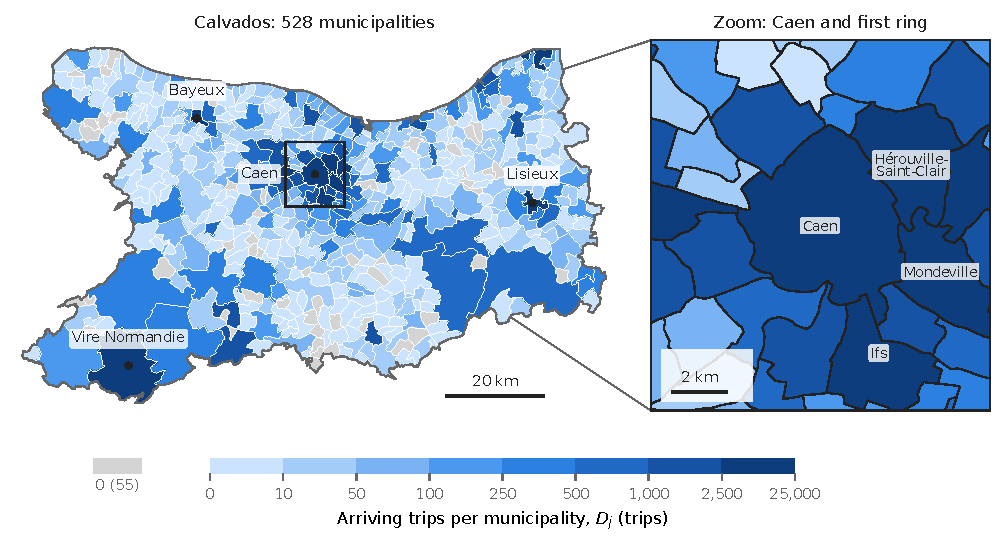
\includegraphics[width=\textwidth]{arrivals_map}
  \caption{Arriving trips \Dj{} per municipality, with URSSAF employment and $N = 126{,}433$. Grey: the 55
  municipalities without URSSAF employees ($\Dj = 0$). Right: zoom on Caen and its first ring. Data: URSSAF
  2019~\cite{urssaf-employment}, \cref{sec:trip-production}; IGN CONTOURS-IRIS 2021~\cite{ign-contours-iris};
  Lambert-93.}
  \label{fig:arrivals-map}
\end{figure}

The arrivals are much more concentrated than the departures (\cref{fig:arrivals-map}). Caen receives 24{,}672 trips
(19.5\,\% of $N$), followed by H\'erouville-Saint-Clair (7{,}783), Mondeville (7{,}350), Vire Normandie (6{,}278) and
Lisieux (5{,}795). These five municipalities receive 41.0\,\% of all trips, and the 30 largest receive 75.5\,\%. The
median is only 11 trips. Caen and its first ring form one dark block on the map. Bayeux, Lisieux, Vire Normandie,
Falaise and the coastal towns of Honfleur and Deauville are isolated dark spots. Most rural municipalities receive fewer
than 50 trips. The large rural \emph{communes nouvelles}, which have the highest production per IRIS
(\cref{fig:trips-per-iris-map}), are only mid-range here: they have many residents but few private jobs.
\textbf{55 municipalities have no URSSAF employee and receive no trip}. 10 of them have no URSSAF record at all, and 45
have a record with 0 employees. They are small villages: MOBPRO counts only 1{,}073 jobs in all of them together
(0.4\,\% of all jobs).

\paragraph{Sensitivity: MOBPRO jobs instead of URSSAF.}
With the MOBPRO jobs (all employed persons, at the place of work), $\sum_j W_j = 275{,}908$, so
$0.7 \sum_j W_j = 193{,}135$. This is still below $0.7 \sum_i \Oi = 204{,}365$, so \textbf{the employment term binds in
both variants}, but $N$ is 1.53 times larger (\cref{tab:attraction-sensitivity}). The spatial pattern is similar: the
\Dj{} of the two variants correlate at $r = 0.971$ ($0.969$ without Caen). The rank correlation is only 0.862, because
small municipalities with few private jobs change rank. The main difference is the public sector. With MOBPRO, Caen
receives 26.6\,\% of the trips instead of 19.5\,\%. With URSSAF, Caen, Bayeux and Lisieux (administration, hospitals,
schools) get only 48--61\,\% of their MOBPRO value. Private employment zones such as Mondeville and Bretteville-sur-Odon
get 7--31\,\% more.

\begin{table}[H]
  \centering
  \caption{Total number of trips $N$ with two sources for the employment $W_j$ (URSSAF private-sector employees,
  MOBPRO jobs). In both cases the employment term of \cref{eq:total-trips-N} is the minimum. $\Dj = 0$: number of
  municipalities without arrivals; Caen: share of $N$ that arrives in Caen.}
  \label{tab:attraction-sensitivity}
  \begin{tabular}{@{}lrrrrrr@{}}
    \toprule
    $W_j$ & $\sum_j W_j$ & $0.7 \sum_j W_j$ & $0.7 \sum_i \Oi$ & $N$ & $\Dj = 0$ & Caen \\
    \midrule
    URSSAF (used) & 180{,}618 & \textbf{126{,}433} & 204{,}365 & \textbf{126{,}433} & 55 & 19.5\,\% \\
    MOBPRO jobs & 275{,}908 & \textbf{193{,}135} & 204{,}365 & 193{,}135 & 7 & 26.6\,\% \\
    \bottomrule
  \end{tabular}
\end{table}

\subsection{Scaling the demand \texorpdfstring{$\Oprime$}{O'} (preparation for Exercise 2.3)}

\paragraph{Method.}
In a balanced model, the total number of originating trips must equal the total number of arriving trips. The demand
of \cref{sec:trip-production} is therefore scaled proportionally to the total $N$:
\begin{equation}\label{eq:scaling}
  \Oprime = N\, \frac{\Oi}{\sum_{i'} O_{i'}} .
\end{equation}
By construction, $\sum_i \Oprime = \sum_j \Dj = N$. Each municipality keeps its share of the trips, so \Oprime{} has
the same spatial pattern as \Oi{}.
\begin{lstlisting}[style=py]
O_scaled = N * O / O.sum()                       # factor N / sum(O) = 0.4331
assert np.isclose(O_scaled.sum(), D.sum())       # both equal N

zones = gdf_municipalities[["municipality_id", "name", "geometry"]].copy()
zones["O"], zones["D"] = O_scaled, D
write_zones(zones)          # checks the contract, writes data/processed/zones.parquet
\end{lstlisting}

\paragraph{Result.}
The scaling factor is $N / \sum_i \Oi = 0.4331$. Caen, for example, goes from 40{,}937 to 17{,}728 departures.
$\sum_i \Oprime = \sum_j \Dj = 126{,}432.6$; the difference is 0.0, also after the file has been written and read back.
Since \Oprime{} and \Dj{} now have the same total, they can be compared per municipality (\cref{fig:net-balance-map}).
471 municipalities have more departures than arrivals, and 57 have more arrivals. The largest surpluses of arrivals
are Caen ($-6{,}944$), Mondeville ($-5{,}517$), H\'erouville-Saint-Clair ($-3{,}947$), Vire Normandie ($-3{,}556$) and
Lisieux ($-2{,}504$). The largest surpluses of departures are rural \emph{communes nouvelles}, led by Souleuvre en
Bocage ($+1{,}057$) and M\'ezidon Vall\'ee d'Auge ($+980$). These are the same five municipalities as the largest net
outflows of the scaled comparison in \cref{sec:territorial-II-difference}. This is the commuting pattern that the
gravity model of \cref{sec:trip-distribution} has to reproduce.

\begin{figure}[H]
  \centering
  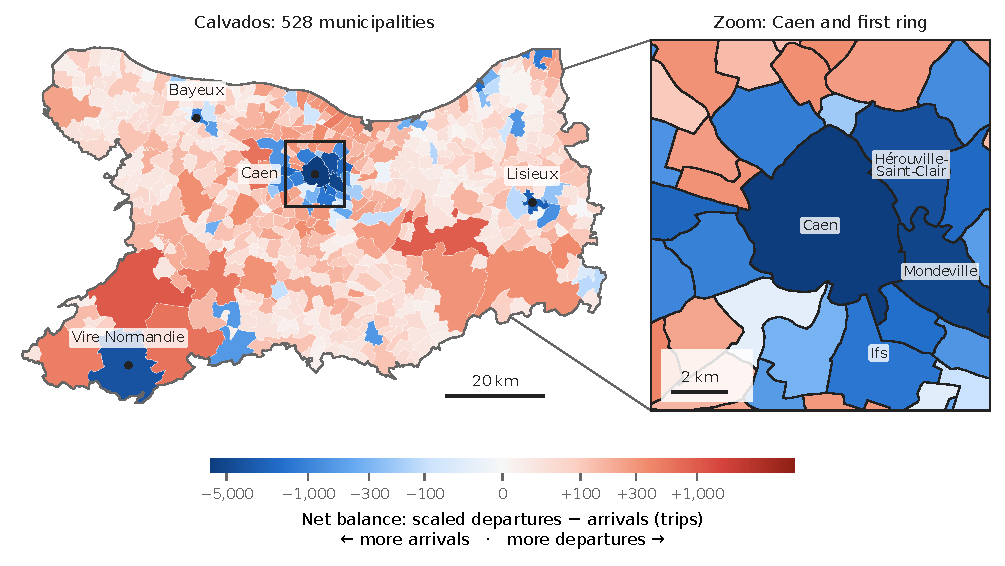
\includegraphics[width=\textwidth]{net_balance_map}
  \caption{Net balance $\Oprime - \Dj$ per municipality (scaled departures minus arrivals, both summing to $N$). Red:
  more departures (residential); blue: more arrivals (employment centres). The colour scale is linear within
  $\pm 100$ trips and logarithmic beyond, as in \cref{sec:territorial-II}.}
  \label{fig:net-balance-map}
\end{figure}

\paragraph{Hand-off file.}
\Oprime{} and \Dj{}, together with the municipality geometry, form the hand-off file
\code{data/processed/zones.parquet}: 528 rows sorted by INSEE code, with the columns \code{municipality\_id},
\code{name}, \code{geometry} (EPSG:2154), \code{O}~$=\Oprime$ and \code{D}~$=\Dj$. It is the only interface to the second part of the project
(\crefrange{sec:trip-distribution}{sec:routing}). The file is written by a function that checks the
contract, and it passes the check after being read back: unique codes identical to the municipality boundaries, no
missing or negative values, and $\sum O = \sum D = N$.

\subsection{Plausibility check with commuting data}\label{sec:trip-attraction-plausibility}

There is no ``true'' value of \Dj{}, but MOBPRO RP2019 \cite{insee-mobpro-2019} counts the real commuters
(\cref{tab:attraction-plausibility}). \textbf{255{,}249 persons} both live and work in Calvados: 171{,}986 between
different municipalities and 83{,}263 within their own municipality. This is 92\,\% of the employed residents and of
the jobs, not 70\,\%. Our $N = 126{,}433$ is therefore only \textbf{49.5\,\% of the real number} (73.5\,\% of the
commuters between different municipalities). With the MOBPRO jobs it would be 75.7\,\%.

\begin{table}[H]
  \centering
  \caption{Scaled departures \Oprime{} and arrivals \Dj{} compared with MOBPRO RP2019, Calvados: ratio of the totals,
  and Pearson ($r$) and Spearman ($\rho$) correlation over the 528 municipalities. ``Within Calvados'': commuters with
  home and work in the department.}
  \label{tab:attraction-plausibility}
  \begin{tabular}{@{}llrrrrr@{}}
    \toprule
    Model & Reference (MOBPRO) & Total & Ratio & $r$ & $r$ excl.\ Caen & $\rho$ \\
    \midrule
    \Dj{} & Jobs at the place of work & 275{,}908 & 0.458 & 0.971 & 0.969 & 0.862 \\
    \Dj{} & Arrivals within Calvados & 255{,}249 & 0.495 & 0.969 & 0.970 & 0.857 \\
    \Oprime{} & Employed residents & 277{,}131 & 0.456 & 0.9995 & 0.9974 & 0.997 \\
    \Oprime{} & Departures within Calvados & 255{,}249 & 0.495 & 0.9992 & 0.9957 & 0.991 \\
    \bottomrule
  \end{tabular}
\end{table}

The spatial pattern is plausible. \Oprime{} follows the real departures almost exactly ($r = 0.9992$). \Dj{} follows
the real arrivals well ($r = 0.969$), but less closely. The five largest real destinations are also the five largest
\Dj{}, and they receive 43.8\,\% of the real arrivals against 41.0\,\% of $D$. Within this group, Caen gets 19.5\,\% of
$D$ but 27.1\,\% of the real arrivals. Mondeville (5.8\,\% against 3.7\,\%), Vire Normandie and
H\'erouville-Saint-Clair are over-weighted, while Lisieux is about right.

For the simulation in \cref{sec:disaggregation,sec:routing}, this means that the model produces about 126{,}000
home-to-work trips, \textbf{about half of the real number}. Traffic volumes on the network will be underestimated by
about a factor of two, and trips into Caen will be too few compared with the private employment zones around it.

\paragraph{Problems encountered.}
\begin{itemize}
  \item \emph{URSSAF covers only private salaried jobs.} The total employment is 65\,\% of the MOBPRO jobs. As a result,
  the employment term determines $N$, which is only 43\,\% of the generated trips and half of the real commuters.
  Towns with many public jobs, Caen above all, get too small a share of the arrivals. We keep URSSAF, as in the course
  notebook and \cref{sec:territorial-II}, and report the MOBPRO variant as a sensitivity analysis.
  \item \emph{Municipalities without URSSAF employees.} 55 municipalities have $W_j = 0$ and therefore $\Dj = 0$. They
  have only 0.4\,\% of the MOBPRO jobs, so the effect on the result is negligible. In \cref{sec:trip-distribution} no
  trip ends there, not even within the municipality, but their residents still depart.
  \item \emph{The 70\,\% rule.} In Calvados, 92\,\% of the employed residents also work in the department. The factor
  0.7 is therefore conservative, and together with the URSSAF coverage it halves the number of trips. We apply the
  formula of the assignment and document the difference above.
\end{itemize}

\section{Trip distribution (Exercise 2.3)}\label{sec:trip-distribution}
\noindent Responsible: Person B. Notebook: \code{notebooks/ex23\_trip\_distribution.ipynb}.

\subsection{Distance matrix (1 point)}

\paragraph{Method.}
The distance matrix $\dij$ contains the Euclidean distances in metres between the centroids of all municipalities of
the study area, computed in the projected CRS EPSG:2154 (Lambert-93). The order of the municipalities is fixed by
\code{zones.parquet}. \todo{Describe the computation (centroids, how the zero diagonal, i.e.\ intra-zonal distance,
is treated) and which zone data the work started from (placeholder or final file of Person A).}

\begin{figure}[H]
  \centering
  \figplaceholder{distance_matrix}
  \caption{\todo{Caption: distance matrix $\dij$ between municipality centroids (in metres).}}
  \label{fig:distance-matrix}
\end{figure}

\paragraph{Result.}
\todo{Comment on the structure of \cref{fig:distance-matrix} (or give a table of a subset of the matrix).}

\subsection{Gravity model and resulting flows (1 point)}

\paragraph{Method.}
A double-constrained gravity model is used. The flow from zone $i$ to zone $j$ is
\begin{equation}\label{eq:gravity}
  \Fij = \frac{\Oprime}{\sum_{j'} a_{j'}\, \rho_{ij'}} \cdot \frac{\Dj}{\sum_{i'} p_{i'}\, \rho_{i'j}} \cdot \rhoij ,
\end{equation}
where $\aj$ and $\pii$ are the attraction and production weighting factors that make the flow matrix match the marginal
distributions of origins and destinations, and $\rhoij$ is the friction term. The origins are the scaled demand
$\Oprime$ of \cref{eq:scaling}. The weighting factors are obtained by iterating
\begin{align}
  \pii &= \frac{\Oprime}{\sum_j a_j\, \rhoij}, \label{eq:balancing-p}\\
  \aj  &= \frac{\Dj}{\sum_i p_i\, \rhoij}, \label{eq:balancing-a}
\end{align}
starting from $p_i = a_j = 1$ until the values stabilise. The friction model is
\begin{equation}\label{eq:friction}
  \rhoij = \exp\!\left(\beta\, \dij + \alpha\right),
\end{equation}
with $\dij$ in metres and the parameters of \cref{tab:gravity-parameters}.

\begin{table}[H]
  \centering
  \caption{Gravity model parameters (Table~2 of the assignment).}
  \label{tab:gravity-parameters}
  \begin{tabular}{@{}lr@{}}
    \toprule
    Parameter & Value \\
    \midrule
    $\beta$ & $-1.1\cdot 10^{-4}$ \\
    $\alpha$ & $-0.4$ \\
    \bottomrule
  \end{tabular}
\end{table}

\todo{Confirm against the assignment PDF that the symbols of the two parameters in \cref{tab:gravity-parameters} and the form of
\cref{eq:friction} are right: the text export of the assignment lost the Greek symbols. Note that a constant factor
$e^{\alpha}$ in $\rhoij$ is absorbed by $\pii$ and $\aj$ and does not change $\Fij$. Describe the stopping
criterion, the number of iterations needed, and the convergence plot or error.}

\paragraph{Verification on the toy example.}
\Cref{tab:toy-inputs,tab:toy-distance,tab:toy-flows} reproduce the toy example of the assignment. With the given distances
and the demand and destination values the implementation must reproduce the flow matrix in \cref{tab:toy-flows} (values
rounded down); this is checked in notebook \code{ex23\_trip\_distribution.ipynb}. Note that the assignment prints $D_1 = 9462$ in
its Table~3, which is a typo: the column sum of \cref{tab:toy-flows} for destination~1 is $420$.

\begin{table}[H]
  \centering
  \caption{Toy example: demand and destinations (Table~3 of the assignment, with the corrected $D_1$).}
  \label{tab:toy-inputs}
  \begin{tabular}{@{}lrrrr@{}}
    \toprule
    Zone & 1 & 2 & 3 & 4 \\
    \midrule
    Origins $\Oi$      & 3396 & 5442 & 43196 & 5681 \\
    Destinations $\Dj$ & 420  & 2294 & 48377 & 6621 \\
    \bottomrule
  \end{tabular}
\end{table}

\begin{table}[H]
  \centering
  \caption{Toy example: distance matrix $\dij$ in metres (Table~4 of the assignment).}
  \label{tab:toy-distance}
  \begin{tabular}{@{}lrrrr@{}}
    \toprule
    $i \backslash j$ & 1 & 2 & 3 & 4 \\
    \midrule
    1 & 0     & 4066  & 6595 & 9462  \\
    2 & 4066  & 0     & 4340 & 10299 \\
    3 & 6595  & 4340  & 0    & 7287  \\
    4 & 9462  & 10299 & 7287 & 0     \\
    \bottomrule
  \end{tabular}
\end{table}

\begin{table}[H]
  \centering
  \caption{Toy example: expected flow matrix $\Fij$, values rounded down (Table~5 of the assignment).}
  \label{tab:toy-flows}
  \begin{tabular}{@{}lrrrr@{}}
    \toprule
    $i \backslash j$ & 1 & 2 & 3 & 4 \\
    \midrule
    1 & 74  & 220  & 2661  & 439  \\
    2 & 61  & 445  & 4415  & 518  \\
    3 & 247 & 1463 & 37659 & 3825 \\
    4 & 38  & 163  & 3640  & 1837 \\
    \bottomrule
  \end{tabular}
\end{table}

\paragraph{Result.}
\todo{Report whether the toy example is reproduced (maximum deviation). Then present the flows $\Fij$ of the study area
as a table (excerpt) or a plot, e.g.\ a heat map or a chord diagram, and report the row and column sums versus
$\Oprime$ and $\Dj$.}

\begin{figure}[H]
  \centering
  \figplaceholder{flow_matrix}
  \caption{\todo{Caption: flow matrix $\Fij$ between municipalities (trips).}}
  \label{fig:flow-matrix}
\end{figure}

\subsection{The ten largest flows (1 point)}

\paragraph{Method.}
\todo{Describe how the ten largest origin--destination pairs are selected (including or excluding intra-zonal flows
$i = j$; state the choice).}

\begin{table}[H]
  \centering
  \caption{\todo{Caption: the ten largest flows between municipalities.}}
  \label{tab:top10-flows}
  \begin{tabular}{@{}rllr@{}}
    \toprule
    Rank & Origin & Destination & Flow $\Fij$ \\
    \midrule
    1  & \todo{name} & \todo{name} & \todo{value} \\
    2  & \todo{name} & \todo{name} & \todo{value} \\
    \multicolumn{4}{c}{\todo{\dots rows 3 to 10}} \\
    \bottomrule
  \end{tabular}
\end{table}

\paragraph{Result.}
\todo{Name the pairs and comment on \cref{tab:top10-flows}: role of the largest municipalities, intra-zonal flows,
effect of distance.}

\paragraph{Problems encountered.}
\todo{Document problems, e.g.\ the typo in the toy example, non-convergence if $\sum_i \Oprime \neq \sum_j \Dj$,
zero or very small distances, zones with $\Dj = 0$, runtime of the matrix computation.}

\section{Disaggregation (Exercise 3.1)}\label{sec:disaggregation}
\noindent Responsible: Person B. Notebook: \code{notebooks/B2\_disaggregation.ipynb}.

\subsection{Individual trips and map of origin--destination lines (2 points)}

\paragraph{Method.}
The flow matrix $\Fij$ of \cref{sec:trip-distribution} is converted into a probability matrix
\begin{equation}\label{eq:probability-matrix}
  P_{ij} = \frac{\Fij}{\sum_{i'}\sum_{j'} F_{i'j'}}, \qquad \sum_{i,j} P_{ij} = 1,
\end{equation}
from which $n$ origin--destination pairs are sampled with replacement, with $n \ge 10\,000$. For each pair, a random
origin coordinate and a random destination coordinate are drawn from within the respective zones. The departure time of
each trip is sampled as described in the next subsection.
\todo{State $n$, the random seed (from \code{lsm.config}), how random points inside a polygon are drawn (e.g.\ rejection
sampling in the bounding box) and whether the sampled coordinates are drawn uniformly in the municipality or restricted
(e.g.\ to built-up areas).}

\begin{figure}[H]
  \centering
  \figplaceholder{trips_map}
  \caption{\todo{Caption: generated trips drawn as lines from origin to destination.}}
  \label{fig:trips-map}
\end{figure}

\paragraph{Result.}
\todo{Describe \cref{fig:trips-map}. Check that the sampled origin--destination counts per zone pair are consistent
with $\Fij$ (e.g.\ correlation or relative error of the aggregated sample against \cref{eq:probability-matrix}).}

\subsection{Distribution of the departure times (1 point)}

\paragraph{Method.}
The departure time $T$ (in seconds after midnight) of each trip is drawn from a normal distribution,
\begin{equation}\label{eq:departure-time}
  T \sim \mathcal{N}\!\left(\mu,\, \sigma^{2}\right), \qquad \sigma = 3600\,\mathrm{s},
\end{equation}
and samples with $T < 0$ are reset to $0$.
\todo{Fill in $\mu$ from the assignment PDF: the text export reads ``83600'' for the mean, which looks like a lost
multiplication sign, i.e.\ $8 \cdot 3600 = 28\,800$\,s (08:00). Check and document, and state the share of samples
that were reset to zero.}

\begin{figure}[H]
  \centering
  \figplaceholder{departure_hist}
  \caption{\todo{Caption: distribution of departure times (histogram or CDF).}}
  \label{fig:departure-hist}
\end{figure}

\paragraph{Result.}
\todo{Describe \cref{fig:departure-hist} (peak, spread, share reset to zero, time axis in hours).}

\paragraph{Problems encountered.}
\todo{Document problems, e.g.\ sampling coordinates in non-convex or multi-part polygons, runtime, a spike at zero
caused by the clipping, trips with identical origin and destination zone.}

\section{Routing (Exercise 3.2)}\label{sec:routing}
\noindent Responsible: Person B. Notebook: \code{notebooks/ex32\_routing.ipynb}.

\subsection{Road network from OpenStreetMap (2 points)}

\paragraph{Method.}
\todo{Describe the OpenStreetMap extract \cite{geofabrik-osm} (region file, date), how it was cropped to the study area
(e.g.\ with osmium-tool and a buffered boundary), how the road network was extracted and converted into a routable
graph (pyrosm \cite{pyrosm} or OSMnx \cite{osmnx}; network type, edge attributes used as routing weight, e.g.\ length
or travel time, handling of one-way streets and of the largest connected component), and the number of nodes and edges
(\cref{tab:network-stats}).}

\begin{table}[H]
  \centering
  \caption{\todo{Caption: size of the routing network.}}
  \label{tab:network-stats}
  \begin{tabular}{@{}lr@{}}
    \toprule
    Quantity & Value \\
    \midrule
    Nodes & \todo{value} \\
    Edges & \todo{value} \\
    Total length [km] & \todo{value} \\
    \bottomrule
  \end{tabular}
\end{table}

\begin{figure}[H]
  \centering
  \figplaceholder{network_map}
  \caption{\todo{Caption: road network of the study area.}}
  \label{fig:network-map}
\end{figure}

\paragraph{Result.}
\todo{Describe \cref{fig:network-map}.}

\subsection{Routing of the trips and flow per link (2 points)}

\paragraph{Method.}
\todo{Describe how origin and destination coordinates are mapped to the nearest network node (CRS, distance of the snap),
which shortest-path algorithm and weight are used, how the number of trips traversing each edge is counted, how trips
without a path are handled, and the runtime.}

\begin{figure}[H]
  \centering
  \figplaceholder{edge_flows_map}
  \caption{\todo{Caption: number of trips per network link.}}
  \label{fig:edge-flows-map}
\end{figure}

\paragraph{Result.}
\todo{Report the number of routed trips, trips without a route, and the most loaded links, and comment on
\cref{fig:edge-flows-map} (major roads, bottlenecks, bridges, effect of the border of the study area).}

\paragraph{Problems encountered.}
\todo{Document problems, e.g.\ the extract is larger than the study area, unreachable nodes, long runtimes,
memory, the network ends at the border of the department although trips cross it.}

\section{Discussion}\label{sec:discussion}

\subsection{Limitations}
\todo{Discuss the main modelling limitations: a single trip-purpose model with one growth factor per SPC and no mode
choice; trips limited to the study area through the 70\,\% rule; friction with fixed parameters instead of estimated
ones; centroid-to-centroid distances and intra-zonal distance zero; employment taken from private-sector URSSAF data
only; municipalities as zones; random coordinates uniform in the zone; shortest paths without congestion.}

\subsection{Consistency checks across the pipeline}
\todo{Document the checks: $\sum_i \Oprime = \sum_j \Dj = N$; row and column sums of $\Fij$ match $\Oprime$ and $\Dj$;
number of sampled trips per zone pair versus $\Fij$; every sampled trip is routed; municipality identifiers are
identical in all hand-off files.}

\begin{table}[H]
  \centering
  \caption{\todo{Caption: consistency checks along the pipeline.}}
  \label{tab:consistency-checks}
  \begin{tabular}{@{}llr@{}}
    \toprule
    Check & Expected & Observed \\
    \midrule
    $\sum_i \Oprime$ versus $\sum_j \Dj$ & equal & \todo{value} \\
    $\sum_j \Fij$ versus $\Oprime$ (max.\ deviation) & $\approx 0$ & \todo{value} \\
    $\sum_i \Fij$ versus $\Dj$ (max.\ deviation) & $\approx 0$ & \todo{value} \\
    Routed trips versus generated trips & equal & \todo{value} \\
    \bottomrule
  \end{tabular}
\end{table}

\subsection{Overview of the problems encountered}
\todo{Summarise the problems documented at the end of each exercise (\cref{sec:study-area,sec:territorial-I,sec:territorial-II,sec:trip-production,sec:trip-attraction,sec:trip-distribution,sec:disaggregation,sec:routing}),
how they were solved and what remains open. The assignment gives partial points for documented problems.}

\subsection{Possible extensions}
\todo{Optional: finer zones (IRIS), estimated friction, mode choice, time-dependent routing, validation against the INSEE
commuting flows.}


%% ---------------------------------------------------------------------------
%% BIBLIOGRAPHY
%% ---------------------------------------------------------------------------
\bibliographystyle{IEEEtran}
\bibliography{bibliography/references}

%% ---------------------------------------------------------------------------
%% APPENDICES
%% ---------------------------------------------------------------------------
\appendix
\section{Reproducibility}\label{sec:appendix-reproducibility}

\subsection{Repository structure}
\todo{Add the repository URL (also in \code{main.tex}, \code{\textbackslash repourl}) and the commit hash of the
submitted version.}

\begin{table}[H]
  \centering
  \caption{Repository structure.}
  \label{tab:repo-structure}
  \begin{tabularx}{\textwidth}{@{}lX@{}}
    \toprule
    Path & Content \\
    \midrule
    \code{README.md}                  & Project overview, team split, how to run \\
    \code{environment.yml}            & Conda environment \\
    \code{data/raw/}                  & Downloaded data sets (not in Git) \\
    \code{data/processed/}            & Intermediate files, including \code{zones.parquet} (not in Git) \\
    \code{data/DATA\_SOURCES.md}      & Download links and known pitfalls \\
    \code{src/lsm/}                   & Shared package: configuration, loaders, geometry, gravity model, plotting \\
    \code{notebooks/A1}--\code{A4}    & Exercises 1.1 to 2.2 (Person A) \\
    \code{notebooks/B1}--\code{B3}    & Exercises 2.3 to 3.2 (Person B) \\
    \code{tests/}                     & Toy example of the gravity model \\
    \code{report/}                    & This report \\
    \bottomrule
  \end{tabularx}
\end{table}

\subsection{Hand-off between the two parts}
The file \code{data/processed/zones.parquet} is the only interface between Person A and Person B. It contains one row
per municipality with the columns \code{municipality\_id} (string, INSEE code), \code{name} (string),
\code{geometry} (EPSG:2154), \code{O} (float, the scaled demand \Oprime) and \code{D} (float, \Dj), with the constraint
$\sum_i \Oprime = \sum_j \Dj = N$.

\subsection{Commands}
\begin{lstlisting}[language=bash]
conda env create -f environment.yml
conda activate lsm
pip install -e .            # or: put src/ on sys.path (done in the notebooks)
pytest                      # toy example of the gravity model
# run the notebooks in the order A1, A2, A3, A4, B1, B2, B3
cd report && ./build.sh     # or .\build.ps1 on Windows -> report/build/main.pdf
\end{lstlisting}

\subsection{Versions and seeds}
\todo{List the software versions (Python, geopandas, OSMnx, pyrosm, \dots; output of \code{conda list}), the date and
version of each data set, and the random seed(s) used for the disaggregation (see \code{src/lsm/config.py}).}

\begin{table}[H]
  \centering
  \caption{Versions and seeds.}
  \label{tab:versions}
  \begin{tabular}{@{}ll@{}}
    \toprule
    Item & Value \\
    \midrule
    Python & \todo{version} \\
    geopandas, OSMnx, pyrosm & \todo{versions} \\
    Random seed & \todo{value from \code{config.py}} \\
    Census / IRIS / URSSAF / OSM vintage & \todo{dates} \\
    \bottomrule
  \end{tabular}
\end{table}

\subsection{Additional tables and figures}
\todo{Extra tables that do not fit in the main text, e.g.\ the full list of municipalities with their statistics.}


\end{document}
